% Options for packages loaded elsewhere
\PassOptionsToPackage{unicode}{hyperref}
\PassOptionsToPackage{hyphens}{url}
%
\documentclass[
]{article}
\usepackage{amsmath,amssymb}
\usepackage{lmodern}
\usepackage{iftex}
\ifPDFTeX
  \usepackage[T1]{fontenc}
  \usepackage[utf8]{inputenc}
  \usepackage{textcomp} % provide euro and other symbols
\else % if luatex or xetex
  \usepackage{unicode-math}
  \defaultfontfeatures{Scale=MatchLowercase}
  \defaultfontfeatures[\rmfamily]{Ligatures=TeX,Scale=1}
\fi
% Use upquote if available, for straight quotes in verbatim environments
\IfFileExists{upquote.sty}{\usepackage{upquote}}{}
\IfFileExists{microtype.sty}{% use microtype if available
  \usepackage[]{microtype}
  \UseMicrotypeSet[protrusion]{basicmath} % disable protrusion for tt fonts
}{}
\makeatletter
\@ifundefined{KOMAClassName}{% if non-KOMA class
  \IfFileExists{parskip.sty}{%
    \usepackage{parskip}
  }{% else
    \setlength{\parindent}{0pt}
    \setlength{\parskip}{6pt plus 2pt minus 1pt}}
}{% if KOMA class
  \KOMAoptions{parskip=half}}
\makeatother
\usepackage{xcolor}
\usepackage[margin=1in]{geometry}
\usepackage{color}
\usepackage{fancyvrb}
\newcommand{\VerbBar}{|}
\newcommand{\VERB}{\Verb[commandchars=\\\{\}]}
\DefineVerbatimEnvironment{Highlighting}{Verbatim}{commandchars=\\\{\}}
% Add ',fontsize=\small' for more characters per line
\usepackage{framed}
\definecolor{shadecolor}{RGB}{248,248,248}
\newenvironment{Shaded}{\begin{snugshade}}{\end{snugshade}}
\newcommand{\AlertTok}[1]{\textcolor[rgb]{0.94,0.16,0.16}{#1}}
\newcommand{\AnnotationTok}[1]{\textcolor[rgb]{0.56,0.35,0.01}{\textbf{\textit{#1}}}}
\newcommand{\AttributeTok}[1]{\textcolor[rgb]{0.77,0.63,0.00}{#1}}
\newcommand{\BaseNTok}[1]{\textcolor[rgb]{0.00,0.00,0.81}{#1}}
\newcommand{\BuiltInTok}[1]{#1}
\newcommand{\CharTok}[1]{\textcolor[rgb]{0.31,0.60,0.02}{#1}}
\newcommand{\CommentTok}[1]{\textcolor[rgb]{0.56,0.35,0.01}{\textit{#1}}}
\newcommand{\CommentVarTok}[1]{\textcolor[rgb]{0.56,0.35,0.01}{\textbf{\textit{#1}}}}
\newcommand{\ConstantTok}[1]{\textcolor[rgb]{0.00,0.00,0.00}{#1}}
\newcommand{\ControlFlowTok}[1]{\textcolor[rgb]{0.13,0.29,0.53}{\textbf{#1}}}
\newcommand{\DataTypeTok}[1]{\textcolor[rgb]{0.13,0.29,0.53}{#1}}
\newcommand{\DecValTok}[1]{\textcolor[rgb]{0.00,0.00,0.81}{#1}}
\newcommand{\DocumentationTok}[1]{\textcolor[rgb]{0.56,0.35,0.01}{\textbf{\textit{#1}}}}
\newcommand{\ErrorTok}[1]{\textcolor[rgb]{0.64,0.00,0.00}{\textbf{#1}}}
\newcommand{\ExtensionTok}[1]{#1}
\newcommand{\FloatTok}[1]{\textcolor[rgb]{0.00,0.00,0.81}{#1}}
\newcommand{\FunctionTok}[1]{\textcolor[rgb]{0.00,0.00,0.00}{#1}}
\newcommand{\ImportTok}[1]{#1}
\newcommand{\InformationTok}[1]{\textcolor[rgb]{0.56,0.35,0.01}{\textbf{\textit{#1}}}}
\newcommand{\KeywordTok}[1]{\textcolor[rgb]{0.13,0.29,0.53}{\textbf{#1}}}
\newcommand{\NormalTok}[1]{#1}
\newcommand{\OperatorTok}[1]{\textcolor[rgb]{0.81,0.36,0.00}{\textbf{#1}}}
\newcommand{\OtherTok}[1]{\textcolor[rgb]{0.56,0.35,0.01}{#1}}
\newcommand{\PreprocessorTok}[1]{\textcolor[rgb]{0.56,0.35,0.01}{\textit{#1}}}
\newcommand{\RegionMarkerTok}[1]{#1}
\newcommand{\SpecialCharTok}[1]{\textcolor[rgb]{0.00,0.00,0.00}{#1}}
\newcommand{\SpecialStringTok}[1]{\textcolor[rgb]{0.31,0.60,0.02}{#1}}
\newcommand{\StringTok}[1]{\textcolor[rgb]{0.31,0.60,0.02}{#1}}
\newcommand{\VariableTok}[1]{\textcolor[rgb]{0.00,0.00,0.00}{#1}}
\newcommand{\VerbatimStringTok}[1]{\textcolor[rgb]{0.31,0.60,0.02}{#1}}
\newcommand{\WarningTok}[1]{\textcolor[rgb]{0.56,0.35,0.01}{\textbf{\textit{#1}}}}
\usepackage{longtable,booktabs,array}
\usepackage{calc} % for calculating minipage widths
% Correct order of tables after \paragraph or \subparagraph
\usepackage{etoolbox}
\makeatletter
\patchcmd\longtable{\par}{\if@noskipsec\mbox{}\fi\par}{}{}
\makeatother
% Allow footnotes in longtable head/foot
\IfFileExists{footnotehyper.sty}{\usepackage{footnotehyper}}{\usepackage{footnote}}
\makesavenoteenv{longtable}
\usepackage{graphicx}
\makeatletter
\def\maxwidth{\ifdim\Gin@nat@width>\linewidth\linewidth\else\Gin@nat@width\fi}
\def\maxheight{\ifdim\Gin@nat@height>\textheight\textheight\else\Gin@nat@height\fi}
\makeatother
% Scale images if necessary, so that they will not overflow the page
% margins by default, and it is still possible to overwrite the defaults
% using explicit options in \includegraphics[width, height, ...]{}
\setkeys{Gin}{width=\maxwidth,height=\maxheight,keepaspectratio}
% Set default figure placement to htbp
\makeatletter
\def\fps@figure{htbp}
\makeatother
\setlength{\emergencystretch}{3em} % prevent overfull lines
\providecommand{\tightlist}{%
  \setlength{\itemsep}{0pt}\setlength{\parskip}{0pt}}
\setcounter{secnumdepth}{5}
\usepackage{booktabs}
\ifLuaTeX
  \usepackage{selnolig}  % disable illegal ligatures
\fi
\usepackage[]{natbib}
\bibliographystyle{plainnat}
\IfFileExists{bookmark.sty}{\usepackage{bookmark}}{\usepackage{hyperref}}
\IfFileExists{xurl.sty}{\usepackage{xurl}}{} % add URL line breaks if available
\urlstyle{same} % disable monospaced font for URLs
\hypersetup{
  pdftitle={Initiation au langage R},
  pdfauthor={Cédric HASSEN-KHODJA},
  hidelinks,
  pdfcreator={LaTeX via pandoc}}

\title{Initiation au langage R}
\author{Cédric HASSEN-KHODJA}
\date{}

\begin{document}
\maketitle

{
\setcounter{tocdepth}{2}
\tableofcontents
}
\hypertarget{r}{%
\section{R}\label{r}}

\hypertarget{quest-ce-que-le-logiciel-r}{%
\subsection{Qu'est-ce que le logiciel R ?}\label{quest-ce-que-le-logiciel-r}}

R\footnote{\url{http://www.r-project.org/}} est un \textbf{langage de programmation} et un \textbf{environnement de développement} (posit)
utilisés pour le calcul statistique et la visualisation des données. Il est largement
utilisé par les scientifiques, les analystes et les développeurs pour \textbf{analyser et visualiser des données, développer des applications et créer des algorithmes}.
Il offre une variété de fonctionnalités, notamment des outils pour le traitement
et la manipulation de données, des \textbf{packages} pour le traitement des données et des bibliothèques pour le traitement des données.

R est disponible pour de nombreuses plateformes, notamment \textbf{Windows, Mac OS X et Linux}.
Il est également disponible sous forme de packages pour les systèmes d'exploitation populaires, tels que Ubuntu, Red Hat et Debian.

\hypertarget{installer-r}{%
\subsection{Installer R}\label{installer-r}}

Pour installer R sous Windows, Linux ou macOS vous devez d'abord télécharger le package d'installation à partir du \textbf{site Web officiel de R (CRAN)} ou sur un de ses miroir\footnote{miroir basé à Lyon, \url{https://pbil.univ-lyon1.fr/CRAN/}}.\\

\begin{itemize}
\tightlist
\item
  Sous Windows ou sous MacOS, une fois le package téléchargé, double-cliquez sur le fichier d'installation et suivez les instructions à l'écran pour compléter l'installation.\\
\item
  Sous Linux\footnote{\url{https://pbil.univ-lyon1.fr/CRAN/bin/linux/}}, suivez les instructions à l'écran pour faire l'installation de R.
\end{itemize}

\hypertarget{rstudio-desktop}{%
\subsection{RStudio Desktop}\label{rstudio-desktop}}

RStudio Desktop est une application de bureau qui offre une \textbf{interface utilisateur graphique} (GUI) pour le
langage de programmation R. Il fournit un \textbf{environnement de développement} intuitif pour le codage, le débogage et la visualisation des données. Il offre également des outils pour l'analyse statistique, le traitement des données et la génération de rapports. RStudio Desktop\footnote{\url{https://posit.co/download/rstudio-desktop/}} est disponible pour Windows, Mac OS X et Linux.\\
Pour avoir un aperçu des différentes possibilités qu'offre l'interface vous pouvez récupérer le cheat sheet\footnote{\url{https://raw.githubusercontent.com/rstudio/cheatsheets/main/rstudio-ide.pdf}} dédié.

Pour commencer, vous pouvez créer un nouveau projet R en utilisant le menu \textbf{File \textgreater{} New project}. Dans
la fenêtre suivante, choisissez \textbf{New directory} pour créer un répertoire de travail sur votre ordinateur ou
\textbf{Open directory} si vous avez déjà un répertoire de travail. Dans la fenêtre suivante, choisissez \textbf{New Project} et créez un répertoire \textbf{MyFirstProject} sur le bureau (ou ailleurs) et validez par \textbf{Create Project}.\\

\begin{figure}
\centering
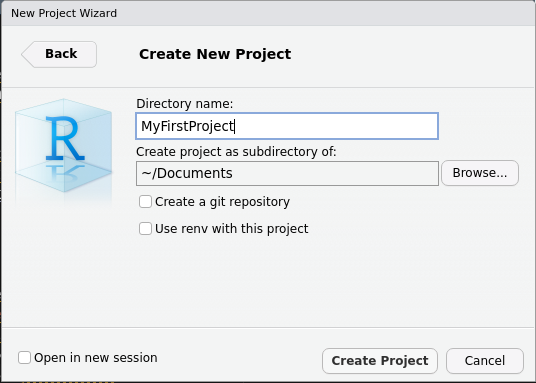
\includegraphics{~/Images/new_project.png}
\caption{Voici un nouveau projet !}
\end{figure}

Créez un nouveau script R à l'intérieur du projet \textbf{MyFirstProject} en utilisant \textbf{File -\textgreater{} New File} et
choisissez \textbf{Rscript}. Le nouveau script est ouvert dans une fenêtre \textbf{Untitled1}. Pour
l'enregistrer, utilisez \textbf{File -\textgreater{} Save as} et donnez-lui un nom, par exemple \textbf{MyFirstScript}.\\
Il est automatiquement enregistré dans le répertoire MyFirstProject. Fermez RStudio avec \textbf{File -\textgreater{} Quit Session}.~

\begin{figure}
\centering
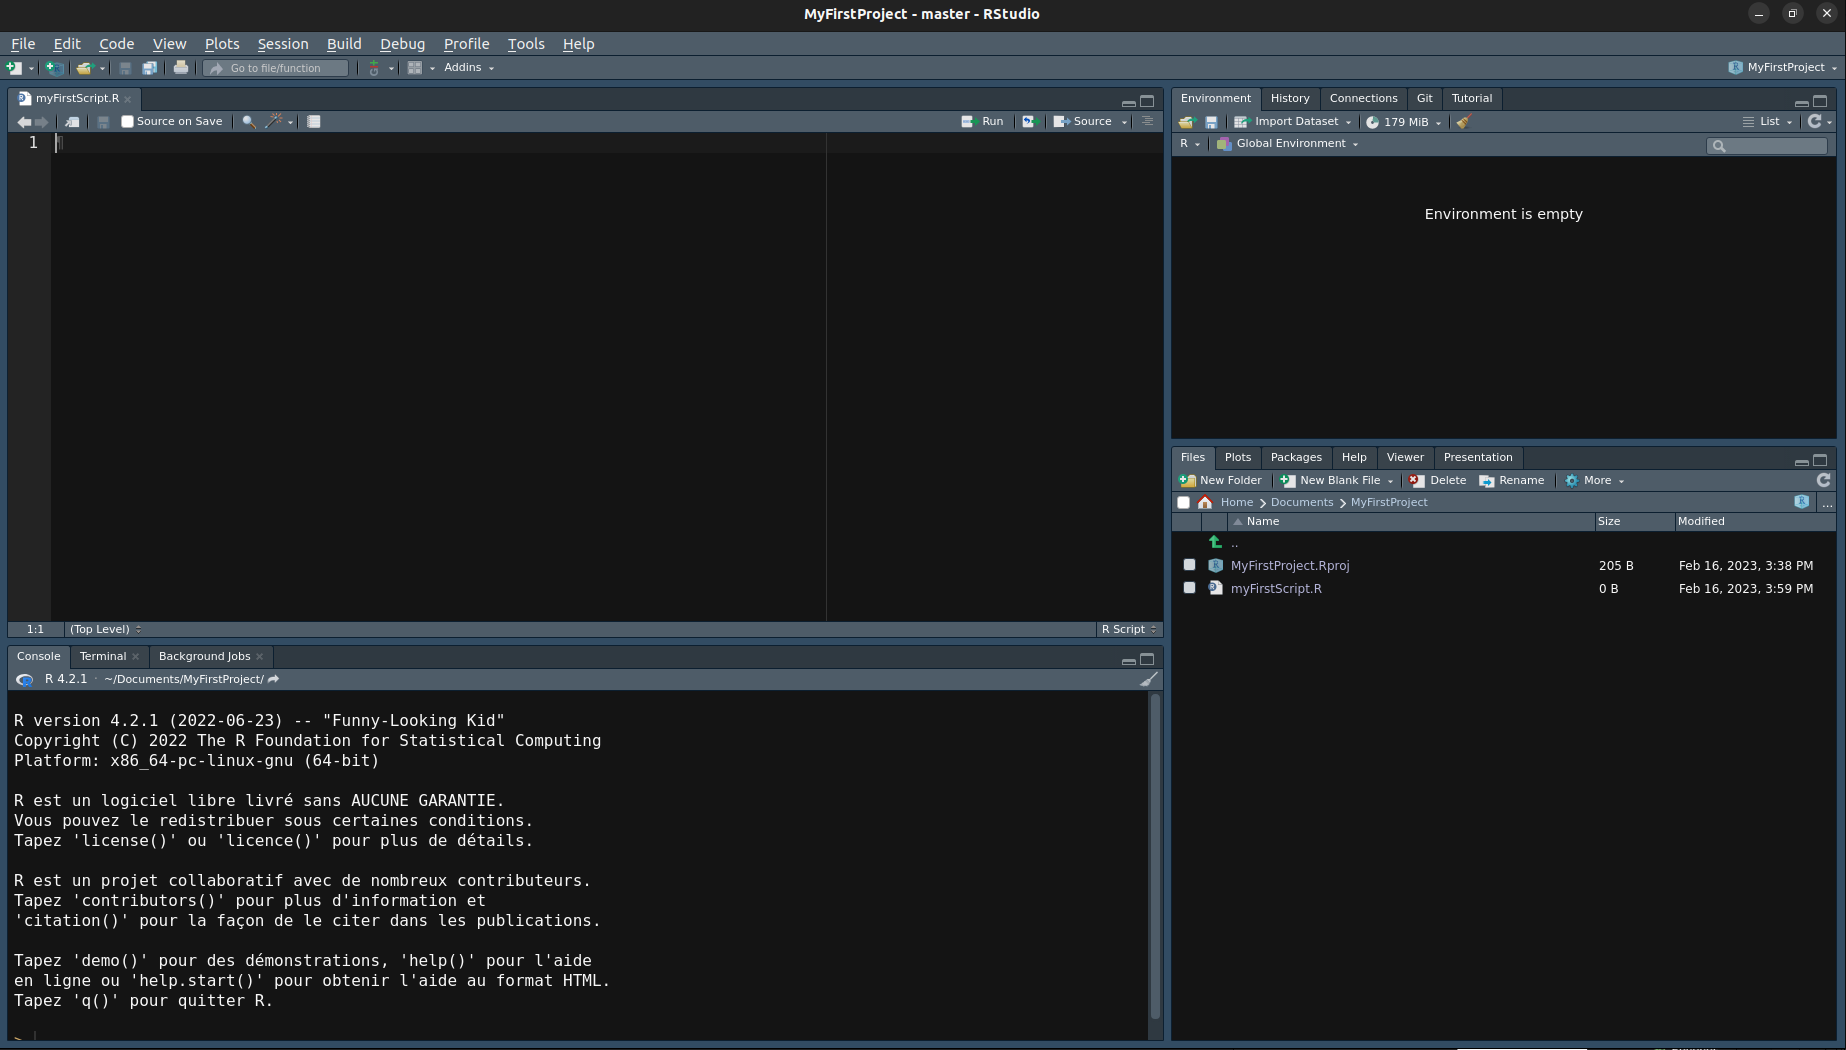
\includegraphics{~/Images/myFirstScript.png}
\caption{Mon premier script !}
\end{figure}

Vérifiez que dans le répertoire MyFirstProject vous avez maintenant ces trois éléments :

\begin{itemize}
\tightlist
\item
  un dossier .Rproj.user
\item
  un fichier MyFirstProject.Rproj
\item
  un script myFirstScript.R
\end{itemize}

\hypertarget{quelques-commandes-de-base-r}{%
\subsection{Quelques commandes de base R}\label{quelques-commandes-de-base-r}}

\begin{quote}
\begin{itemize}
\tightlist
\item
  install.packages() : installe un package R.
\item
  library() : charge un package R.
\item
  search() : recherche un package R.
\item
  update.packages() : met à jour un package R.
\item
  remove.packages() : supprime un package R.
\item
  options() : affiche les options de configuration R.
\item
  setwd() : définit le répertoire de travail R.
\item
  getwd() : affiche le répertoire de travail R.
\item
  save.image() : sauvegarde l'environnement R.
\end{itemize}
\end{quote}

Voici les sorties de quelques commandes pré-citées :

\begin{Shaded}
\begin{Highlighting}[]
\FunctionTok{install.packages}\NormalTok{(}\StringTok{"dplyr"}\NormalTok{)}
\end{Highlighting}
\end{Shaded}

\begin{verbatim}
## Error in install.packages : Updating loaded packages
\end{verbatim}

\begin{Shaded}
\begin{Highlighting}[]
\FunctionTok{library}\NormalTok{(}\StringTok{"dplyr"}\NormalTok{)}
\FunctionTok{getwd}\NormalTok{()}
\end{Highlighting}
\end{Shaded}

\begin{verbatim}
## [1] "/home/cedric/Documents/FormationR _Banyuls"
\end{verbatim}

\hypertarget{le-langage-r}{%
\section{Le langage R}\label{le-langage-r}}

\hypertarget{eluxe9ment-de-base-du-langage-le-vecteur}{%
\subsection{Elément de base du langage : le vecteur}\label{eluxe9ment-de-base-du-langage-le-vecteur}}

Les vecteurs sous R sont des objets unidimensionnels qui contiennent des \textbf{éléments de même type}
(numériques, chaînes de caractères, etc.). Ils sont créés à l'aide de la fonction c() et peuvent être modifiés
à l'aide des opérateurs arithmétiques et des fonctions spécifiques. Les vecteurs peuvent également être indexés
et manipulés à l'aide de fonctions comme subset(), sort(), et merge(). Les vecteurs sont une partie
essentielle de la programmation en R et sont très utiles pour stocker et manipuler des données.

\begin{enumerate}
\def\labelenumi{\arabic{enumi}.}
\tightlist
\item
  Utiliser la fonction \texttt{c()} pour créer un vecteur à partir d'une liste:
\end{enumerate}

\begin{Shaded}
\begin{Highlighting}[]
\NormalTok{v1 }\OtherTok{\textless{}{-}} \FunctionTok{c}\NormalTok{(}\DecValTok{1}\NormalTok{, }\DecValTok{2}\NormalTok{, }\DecValTok{3}\NormalTok{, }\DecValTok{4}\NormalTok{, }\DecValTok{5}\NormalTok{)}
\NormalTok{v1}
\end{Highlighting}
\end{Shaded}

\begin{verbatim}
## [1] 1 2 3 4 5
\end{verbatim}

\begin{enumerate}
\def\labelenumi{\arabic{enumi}.}
\setcounter{enumi}{1}
\tightlist
\item
  Utiliser la fonction \texttt{seq()} pour créer un vecteur de valeurs entières:
\end{enumerate}

\begin{Shaded}
\begin{Highlighting}[]
\NormalTok{v2 }\OtherTok{\textless{}{-}} \FunctionTok{seq}\NormalTok{(}\DecValTok{1}\NormalTok{, }\DecValTok{10}\NormalTok{)}
\NormalTok{v2}
\end{Highlighting}
\end{Shaded}

\begin{verbatim}
##  [1]  1  2  3  4  5  6  7  8  9 10
\end{verbatim}

\begin{enumerate}
\def\labelenumi{\arabic{enumi}.}
\setcounter{enumi}{2}
\tightlist
\item
  Utiliser la fonction \texttt{rep()} pour créer un vecteur avec des valeurs répétées:
\end{enumerate}

\begin{Shaded}
\begin{Highlighting}[]
\NormalTok{v3 }\OtherTok{\textless{}{-}} \FunctionTok{rep}\NormalTok{(}\DecValTok{1}\NormalTok{, }\DecValTok{5}\NormalTok{)}
\NormalTok{v3}
\end{Highlighting}
\end{Shaded}

\begin{verbatim}
## [1] 1 1 1 1 1
\end{verbatim}

\begin{enumerate}
\def\labelenumi{\arabic{enumi}.}
\setcounter{enumi}{3}
\tightlist
\item
  Utiliser la fonction \texttt{seq\_len()} pour créer un vecteur avec des valeurs équidistantes:
\end{enumerate}

\begin{Shaded}
\begin{Highlighting}[]
\NormalTok{v4 }\OtherTok{\textless{}{-}} \FunctionTok{seq\_len}\NormalTok{(}\DecValTok{5}\NormalTok{)}
\end{Highlighting}
\end{Shaded}

\begin{enumerate}
\def\labelenumi{\arabic{enumi}.}
\setcounter{enumi}{4}
\tightlist
\item
  Utiliser la fonction \texttt{vector()} pour créer un vecteur vide:
\end{enumerate}

\begin{Shaded}
\begin{Highlighting}[]
\NormalTok{v5 }\OtherTok{\textless{}{-}} \FunctionTok{vector}\NormalTok{()}
\NormalTok{v5}
\end{Highlighting}
\end{Shaded}

\begin{verbatim}
## logical(0)
\end{verbatim}

\begin{enumerate}
\def\labelenumi{\arabic{enumi}.}
\setcounter{enumi}{5}
\tightlist
\item
  La fonction \texttt{length()} permet de connaître la \emph{taille} d'un vecteur. La fonction \texttt{mode()} permet de connaître le \emph{type} d'un vecteur:
\end{enumerate}

\begin{Shaded}
\begin{Highlighting}[]
\NormalTok{v4 }\OtherTok{\textless{}{-}} \FunctionTok{seq\_len}\NormalTok{(}\DecValTok{5}\NormalTok{)}
\FunctionTok{length}\NormalTok{(v4)}
\end{Highlighting}
\end{Shaded}

\begin{verbatim}
## [1] 5
\end{verbatim}

\begin{Shaded}
\begin{Highlighting}[]
\FunctionTok{mode}\NormalTok{(v4)}
\end{Highlighting}
\end{Shaded}

\begin{verbatim}
## [1] "numeric"
\end{verbatim}

\begin{enumerate}
\def\labelenumi{\arabic{enumi}.}
\setcounter{enumi}{6}
\tightlist
\item
  Pour sélectionner un élément d'un vecteur vous pouvez utiliser les \texttt{{[}{]}} en spécifiant l'index. Si vous souhaitez extraire plusieurs éléments, il faut utiliser la fonction de concaténation \texttt{c()}. Exemple:
\end{enumerate}

\begin{Shaded}
\begin{Highlighting}[]
\NormalTok{animals }\OtherTok{\textless{}{-}} \FunctionTok{c}\NormalTok{(}\StringTok{"lyon"}\NormalTok{, }\StringTok{"chat"}\NormalTok{, }\StringTok{"oiseau"}\NormalTok{)}
\NormalTok{animals[}\DecValTok{1}\NormalTok{]}
\end{Highlighting}
\end{Shaded}

\begin{verbatim}
## [1] "lyon"
\end{verbatim}

\begin{Shaded}
\begin{Highlighting}[]
\NormalTok{animals[}\FunctionTok{c}\NormalTok{(}\DecValTok{1}\NormalTok{,}\DecValTok{3}\NormalTok{)]}
\end{Highlighting}
\end{Shaded}

\begin{verbatim}
## [1] "lyon"   "oiseau"
\end{verbatim}

Un facteur est un type de données utilisé pour \textbf{stocker des valeurs catégoriques} sous R. Les facteurs sont souvent utilisés pour représenter des variables qualitatives telles que des étiquettes de couleur, des groupes d'âge, des sexes, etc. Les facteurs sont stockés sous forme de nombres entiers, mais peuvent être affichés sous forme de chaînes de caractères.

\begin{enumerate}
\def\labelenumi{\arabic{enumi}.}
\tightlist
\item
  Utiliser la fonction \texttt{factor()} pour créer un facteur à partir d'une liste de chaînes de caractères:
\end{enumerate}

\begin{Shaded}
\begin{Highlighting}[]
\NormalTok{f1 }\OtherTok{\textless{}{-}} \FunctionTok{factor}\NormalTok{(}\FunctionTok{c}\NormalTok{(}\StringTok{"rouge"}\NormalTok{, }\StringTok{"bleu"}\NormalTok{, }\StringTok{"vert"}\NormalTok{))}
\NormalTok{f1}
\end{Highlighting}
\end{Shaded}

\begin{verbatim}
## [1] rouge bleu  vert 
## Levels: bleu rouge vert
\end{verbatim}

\begin{enumerate}
\def\labelenumi{\arabic{enumi}.}
\setcounter{enumi}{1}
\tightlist
\item
  Utiliser la fonction \texttt{as.factor()} pour créer un facteur à partir d'une liste de nombres entiers:
\end{enumerate}

\begin{Shaded}
\begin{Highlighting}[]
\NormalTok{f2 }\OtherTok{\textless{}{-}} \FunctionTok{as.factor}\NormalTok{(}\FunctionTok{c}\NormalTok{(}\DecValTok{1}\NormalTok{, }\DecValTok{2}\NormalTok{, }\DecValTok{3}\NormalTok{))}
\NormalTok{f2}
\end{Highlighting}
\end{Shaded}

\begin{verbatim}
## [1] 1 2 3
## Levels: 1 2 3
\end{verbatim}

\begin{enumerate}
\def\labelenumi{\arabic{enumi}.}
\setcounter{enumi}{2}
\tightlist
\item
  Utiliser la fonction \texttt{cut()} pour créer un facteur à partir d'une liste de nombres:
\end{enumerate}

\begin{Shaded}
\begin{Highlighting}[]
\NormalTok{f3 }\OtherTok{\textless{}{-}} \FunctionTok{cut}\NormalTok{(}\FunctionTok{c}\NormalTok{(}\DecValTok{1}\NormalTok{, }\DecValTok{2}\NormalTok{, }\DecValTok{3}\NormalTok{, }\DecValTok{4}\NormalTok{, }\DecValTok{5}\NormalTok{), }\AttributeTok{breaks =} \FunctionTok{c}\NormalTok{(}\DecValTok{1}\NormalTok{, }\DecValTok{3}\NormalTok{, }\DecValTok{5}\NormalTok{))}
\NormalTok{f3}
\end{Highlighting}
\end{Shaded}

\begin{verbatim}
## [1] <NA>  (1,3] (1,3] (3,5] (3,5]
## Levels: (1,3] (3,5]
\end{verbatim}

\begin{enumerate}
\def\labelenumi{\arabic{enumi}.}
\setcounter{enumi}{3}
\tightlist
\item
  Utiliser la fonction \texttt{levels()} pour définir des niveaux pour un facteur existant:
\end{enumerate}

\begin{Shaded}
\begin{Highlighting}[]
\NormalTok{f4 }\OtherTok{\textless{}{-}} \FunctionTok{factor}\NormalTok{(}\FunctionTok{c}\NormalTok{(}\StringTok{"rouge"}\NormalTok{, }\StringTok{"bleu"}\NormalTok{, }\StringTok{"vert"}\NormalTok{))}
\FunctionTok{levels}\NormalTok{(f4) }\OtherTok{\textless{}{-}} \FunctionTok{c}\NormalTok{(}\StringTok{"rouge"}\NormalTok{, }\StringTok{"jaune"}\NormalTok{, }\StringTok{"vert"}\NormalTok{)}
\NormalTok{f4}
\end{Highlighting}
\end{Shaded}

\begin{verbatim}
## [1] jaune rouge vert 
## Levels: rouge jaune vert
\end{verbatim}

\begin{enumerate}
\def\labelenumi{\arabic{enumi}.}
\setcounter{enumi}{4}
\tightlist
\item
  Utiliser la fonction \texttt{relevel()} pour modifier l'ordre des niveaux d'un facteur existant:
\end{enumerate}

\begin{Shaded}
\begin{Highlighting}[]
\NormalTok{f5 }\OtherTok{\textless{}{-}} \FunctionTok{factor}\NormalTok{(}\FunctionTok{c}\NormalTok{(}\StringTok{"rouge"}\NormalTok{, }\StringTok{"bleu"}\NormalTok{, }\StringTok{"vert"}\NormalTok{))}
\FunctionTok{relevel}\NormalTok{(f5, }\AttributeTok{ref =} \StringTok{"rouge"}\NormalTok{)}
\end{Highlighting}
\end{Shaded}

\begin{verbatim}
## [1] rouge bleu  vert 
## Levels: rouge bleu vert
\end{verbatim}

\hypertarget{opuxe9rations-sur-les-vecteurs}{%
\subsection{Opérations sur les vecteurs}\label{opuxe9rations-sur-les-vecteurs}}

Les opérations sur les vecteurs peuvent être utilisées pour effectuer des \textbf{opérations arithmétiques}, des \textbf{opérations logiques} ou des \textbf{opérations de comparaison}.

\begin{enumerate}
\def\labelenumi{\arabic{enumi}.}
\tightlist
\item
  Utiliser l'opérateur \texttt{+} pour additionner deux vecteurs:
\end{enumerate}

\begin{Shaded}
\begin{Highlighting}[]
\NormalTok{vec1 }\OtherTok{\textless{}{-}} \FunctionTok{c}\NormalTok{(}\DecValTok{1}\NormalTok{, }\DecValTok{2}\NormalTok{, }\DecValTok{3}\NormalTok{)}
\NormalTok{vec2 }\OtherTok{\textless{}{-}} \FunctionTok{c}\NormalTok{(}\DecValTok{4}\NormalTok{, }\DecValTok{5}\NormalTok{, }\DecValTok{6}\NormalTok{)}
\NormalTok{vec1 }\SpecialCharTok{+}\NormalTok{ vec2}
\end{Highlighting}
\end{Shaded}

\begin{verbatim}
## [1] 5 7 9
\end{verbatim}

\begin{enumerate}
\def\labelenumi{\arabic{enumi}.}
\setcounter{enumi}{1}
\tightlist
\item
  Utiliser l'opérateur \texttt{-} pour soustraire deux vecteurs:
\end{enumerate}

\begin{Shaded}
\begin{Highlighting}[]
\NormalTok{vec1 }\OtherTok{\textless{}{-}} \FunctionTok{c}\NormalTok{(}\DecValTok{1}\NormalTok{, }\DecValTok{2}\NormalTok{, }\DecValTok{3}\NormalTok{)}
\NormalTok{vec2 }\OtherTok{\textless{}{-}} \FunctionTok{c}\NormalTok{(}\DecValTok{4}\NormalTok{, }\DecValTok{5}\NormalTok{, }\DecValTok{6}\NormalTok{)}
\NormalTok{vec1 }\SpecialCharTok{{-}}\NormalTok{ vec2}
\end{Highlighting}
\end{Shaded}

\begin{verbatim}
## [1] -3 -3 -3
\end{verbatim}

\begin{enumerate}
\def\labelenumi{\arabic{enumi}.}
\setcounter{enumi}{2}
\tightlist
\item
  Utiliser l'opérateur \texttt{*} pour multiplier deux vecteurs:
\end{enumerate}

\begin{Shaded}
\begin{Highlighting}[]
\NormalTok{vec1 }\OtherTok{\textless{}{-}} \FunctionTok{c}\NormalTok{(}\DecValTok{1}\NormalTok{, }\DecValTok{2}\NormalTok{, }\DecValTok{3}\NormalTok{)}
\NormalTok{vec2 }\OtherTok{\textless{}{-}} \FunctionTok{c}\NormalTok{(}\DecValTok{4}\NormalTok{, }\DecValTok{5}\NormalTok{, }\DecValTok{6}\NormalTok{)}
\NormalTok{vec1 }\SpecialCharTok{*}\NormalTok{ vec2}
\end{Highlighting}
\end{Shaded}

\begin{verbatim}
## [1]  4 10 18
\end{verbatim}

\begin{enumerate}
\def\labelenumi{\arabic{enumi}.}
\setcounter{enumi}{3}
\tightlist
\item
  Utiliser l'opérateur \texttt{\&} pour effectuer un ET logique entre deux vecteurs:
\end{enumerate}

\begin{Shaded}
\begin{Highlighting}[]
\NormalTok{vec1 }\OtherTok{\textless{}{-}} \FunctionTok{c}\NormalTok{(}\ConstantTok{TRUE}\NormalTok{, }\ConstantTok{FALSE}\NormalTok{, }\ConstantTok{TRUE}\NormalTok{)}
\NormalTok{vec2  }\OtherTok{\textless{}{-}} \FunctionTok{c}\NormalTok{(}\ConstantTok{FALSE}\NormalTok{, }\ConstantTok{FALSE}\NormalTok{, }\ConstantTok{TRUE}\NormalTok{)}
\NormalTok{vec1 }\SpecialCharTok{\&}\NormalTok{ vec2}
\end{Highlighting}
\end{Shaded}

\begin{verbatim}
## [1] FALSE FALSE  TRUE
\end{verbatim}

\begin{enumerate}
\def\labelenumi{\arabic{enumi}.}
\setcounter{enumi}{4}
\tightlist
\item
  Utiliser l'opérateur \texttt{\textbar{}} pour effectuer un OU logique entre deux vecteurs:
\end{enumerate}

\begin{Shaded}
\begin{Highlighting}[]
\NormalTok{vec1 }\OtherTok{\textless{}{-}} \FunctionTok{c}\NormalTok{(}\ConstantTok{TRUE}\NormalTok{, }\ConstantTok{FALSE}\NormalTok{, }\ConstantTok{TRUE}\NormalTok{)}
\NormalTok{vec2  }\OtherTok{\textless{}{-}} \FunctionTok{c}\NormalTok{(}\ConstantTok{FALSE}\NormalTok{, }\ConstantTok{FALSE}\NormalTok{, }\ConstantTok{TRUE}\NormalTok{)}
\NormalTok{vec1 }\SpecialCharTok{|}\NormalTok{ vec2}
\end{Highlighting}
\end{Shaded}

\begin{verbatim}
## [1]  TRUE FALSE  TRUE
\end{verbatim}

\begin{enumerate}
\def\labelenumi{\arabic{enumi}.}
\setcounter{enumi}{5}
\tightlist
\item
  Utiliser l'opérateur \texttt{!} pour effectuer un NON logique sur un vecteur:
\end{enumerate}

\begin{Shaded}
\begin{Highlighting}[]
\NormalTok{vec }\OtherTok{\textless{}{-}} \FunctionTok{c}\NormalTok{(}\ConstantTok{TRUE}\NormalTok{, }\ConstantTok{FALSE}\NormalTok{, }\ConstantTok{TRUE}\NormalTok{)}
\SpecialCharTok{!}\NormalTok{vec}
\end{Highlighting}
\end{Shaded}

\begin{verbatim}
## [1] FALSE  TRUE FALSE
\end{verbatim}

\begin{enumerate}
\def\labelenumi{\arabic{enumi}.}
\setcounter{enumi}{6}
\tightlist
\item
  Utiliser l'opérateur \texttt{==} pour vérifier si une valeur est égal à un élément du vecteur:
\end{enumerate}

\begin{Shaded}
\begin{Highlighting}[]
\NormalTok{x }\OtherTok{\textless{}{-}} \FunctionTok{c}\NormalTok{(}\DecValTok{1}\NormalTok{, }\DecValTok{2}\NormalTok{, }\DecValTok{3}\NormalTok{)}
\NormalTok{x }\SpecialCharTok{==} \DecValTok{2}
\end{Highlighting}
\end{Shaded}

\begin{verbatim}
## [1] FALSE  TRUE FALSE
\end{verbatim}

\begin{enumerate}
\def\labelenumi{\arabic{enumi}.}
\setcounter{enumi}{7}
\tightlist
\item
  Utiliser l'opérateur \texttt{\textgreater{}} pour vérifier si une valeur est strictement supérieure à un des éléments du vecteur:
\end{enumerate}

\begin{Shaded}
\begin{Highlighting}[]
\NormalTok{x }\OtherTok{\textless{}{-}} \FunctionTok{c}\NormalTok{(}\DecValTok{1}\NormalTok{, }\DecValTok{2}\NormalTok{, }\DecValTok{3}\NormalTok{)}
\NormalTok{x }\SpecialCharTok{\textgreater{}} \DecValTok{2}
\end{Highlighting}
\end{Shaded}

\begin{verbatim}
## [1] FALSE FALSE  TRUE
\end{verbatim}

\begin{enumerate}
\def\labelenumi{\arabic{enumi}.}
\setcounter{enumi}{8}
\tightlist
\item
  Utiliser l'opérateur \texttt{\textless{}} pour vérifier si une valeur est strictement inférieure à un des éléments du vecteur:
\end{enumerate}

\begin{Shaded}
\begin{Highlighting}[]
\NormalTok{x }\OtherTok{\textless{}{-}} \FunctionTok{c}\NormalTok{(}\DecValTok{1}\NormalTok{, }\DecValTok{2}\NormalTok{, }\DecValTok{3}\NormalTok{)}
\NormalTok{x }\SpecialCharTok{\textless{}} \DecValTok{2}
\end{Highlighting}
\end{Shaded}

\begin{verbatim}
## [1]  TRUE FALSE FALSE
\end{verbatim}

\begin{enumerate}
\def\labelenumi{\arabic{enumi}.}
\setcounter{enumi}{9}
\tightlist
\item
  Utiliser l'opérateur \texttt{\%in\%} pour vérifier si une valeur est incluse dans le vecteur:
\end{enumerate}

\begin{Shaded}
\begin{Highlighting}[]
\NormalTok{x }\OtherTok{\textless{}{-}} \FunctionTok{c}\NormalTok{(}\DecValTok{1}\NormalTok{, }\DecValTok{2}\NormalTok{, }\DecValTok{3}\NormalTok{)}
\DecValTok{2} \SpecialCharTok{\%in\%}\NormalTok{ x}
\end{Highlighting}
\end{Shaded}

\begin{verbatim}
## [1] TRUE
\end{verbatim}

\begin{enumerate}
\def\labelenumi{\arabic{enumi}.}
\setcounter{enumi}{10}
\tightlist
\item
  Utiliser l'opérateur \texttt{\%nin\%} (librairie Hmisc) pour vérifier si une valeur n'est pas incluse dans le vecteur :
\end{enumerate}

\begin{Shaded}
\begin{Highlighting}[]
\FunctionTok{library}\NormalTok{(Hmisc)   }
\NormalTok{x }\OtherTok{\textless{}{-}} \FunctionTok{c}\NormalTok{(}\DecValTok{1}\NormalTok{, }\DecValTok{2}\NormalTok{, }\DecValTok{3}\NormalTok{)   }
\DecValTok{2} \SpecialCharTok{\%nin\%}\NormalTok{ x}
\end{Highlighting}
\end{Shaded}

\begin{verbatim}
## [1] FALSE
\end{verbatim}

\hypertarget{la-matrice-un-objet-uxe0-deux-dimensions}{%
\subsection{La matrice : un objet à deux dimensions}\label{la-matrice-un-objet-uxe0-deux-dimensions}}

Les matrices sont une structure de données importante sous R. Elles sont utilisées pour \textbf{stocker des données qui peuvent être représentées sous forme de tableau à deux dimensions}.

Les matrices sous R peuvent être créées à l'aide des fonctions \texttt{matrix()} et \texttt{cbind()}. Par exemple, pour créer une \emph{matrice 3x3 avec des valeurs de 1 à 9}, vous pouvez utiliser la commande suivante:

\begin{Shaded}
\begin{Highlighting}[]
\NormalTok{mat }\OtherTok{\textless{}{-}} \FunctionTok{matrix}\NormalTok{(}\DecValTok{1}\SpecialCharTok{:}\DecValTok{9}\NormalTok{, }\AttributeTok{nrow =} \DecValTok{3}\NormalTok{, }\AttributeTok{ncol =} \DecValTok{3}\NormalTok{, }\AttributeTok{byrow =} \ConstantTok{TRUE}\NormalTok{)}
\NormalTok{mat}
\end{Highlighting}
\end{Shaded}

\begin{verbatim}
##      [,1] [,2] [,3]
## [1,]    1    2    3
## [2,]    4    5    6
## [3,]    7    8    9
\end{verbatim}

Ceci créerait une matrice 3x3 avec les valeurs 1, 2, 3 dans la première ligne, 4, 5, 6 dans la deuxième ligne et 7, 8, 9 dans la troisième ligne.

Vous pouvez également utiliser la fonction \texttt{cbind()} pour créer une \emph{matrice à partir de vecteurs}. Par exemple, pour créer une matrice 3x3 avec des valeurs de 1 à 9, vous pouvez utiliser la commande suivante:

\begin{Shaded}
\begin{Highlighting}[]
\NormalTok{mat }\OtherTok{\textless{}{-}} \FunctionTok{cbind}\NormalTok{(}\FunctionTok{c}\NormalTok{(}\DecValTok{1}\NormalTok{, }\DecValTok{4}\NormalTok{, }\DecValTok{7}\NormalTok{), }\FunctionTok{c}\NormalTok{(}\DecValTok{2}\NormalTok{, }\DecValTok{5}\NormalTok{, }\DecValTok{8}\NormalTok{), }\FunctionTok{c}\NormalTok{(}\DecValTok{3}\NormalTok{, }\DecValTok{6}\NormalTok{, }\DecValTok{9}\NormalTok{))}
\NormalTok{mat}
\end{Highlighting}
\end{Shaded}

\begin{verbatim}
##      [,1] [,2] [,3]
## [1,]    1    2    3
## [2,]    4    5    6
## [3,]    7    8    9
\end{verbatim}

\hypertarget{la-liste}{%
\subsection{La liste}\label{la-liste}}

Les listes sous R sont très utiles car elles peuvent \textbf{contenir des éléments de différents types} (par exemple, des chaînes de caractères, des nombres, des vecteurs, etc.).

Les listes sous R peuvent être créées à l'aide de la fonction \texttt{list()}. Par exemple, pour créer une \emph{liste avec des valeurs de 1 à 9}, vous pouvez utiliser la commande suivante:

\begin{Shaded}
\begin{Highlighting}[]
\NormalTok{l }\OtherTok{\textless{}{-}} \FunctionTok{list}\NormalTok{(}\DecValTok{1}\NormalTok{, }\DecValTok{2}\NormalTok{, }\DecValTok{3}\NormalTok{, }\DecValTok{4}\NormalTok{, }\DecValTok{5}\NormalTok{, }\DecValTok{6}\NormalTok{, }\DecValTok{7}\NormalTok{, }\DecValTok{8}\NormalTok{, }\DecValTok{9}\NormalTok{)}
\NormalTok{l}
\end{Highlighting}
\end{Shaded}

\begin{verbatim}
## [[1]]
## [1] 1
## 
## [[2]]
## [1] 2
## 
## [[3]]
## [1] 3
## 
## [[4]]
## [1] 4
## 
## [[5]]
## [1] 5
## 
## [[6]]
## [1] 6
## 
## [[7]]
## [1] 7
## 
## [[8]]
## [1] 8
## 
## [[9]]
## [1] 9
\end{verbatim}

Les listes sous R peuvent également \textbf{être indexées et manipulées facilement}. Par exemple, pour extraire le premier élément de la liste précédente, vous pouvez utiliser la commande suivante:

\begin{Shaded}
\begin{Highlighting}[]
\NormalTok{first\_element }\OtherTok{\textless{}{-}}\NormalTok{ l[}\DecValTok{1}\NormalTok{]}
\NormalTok{first\_element}
\end{Highlighting}
\end{Shaded}

\begin{verbatim}
## [[1]]
## [1] 1
\end{verbatim}

\hypertarget{le-tableau-de-donnuxe9es}{%
\subsection{Le tableau de données}\label{le-tableau-de-donnuxe9es}}

Les data.frame sous R sont une structure de données très importante pour le \textbf{traitement des données}. Les data.frame sont des objets qui contiennent des données organisées sous \textbf{forme de tableau}, avec \emph{des lignes et des colonnes}. Les lignes représentent des \emph{enregistrements} et les colonnes des \emph{variables}. Les data.frame sont très flexibles et peuvent contenir des \textbf{données de différents types}, y compris des chaînes de caractères, des entiers, des nombres réels, des dates, etc. Les data.frame sont très faciles à \textbf{manipuler, à trier et à filtrer}. On peut également facilement effectuer des \textbf{opérations de jointure} entre deux data.frame.\\
Vous pouvez utiliser la commande \texttt{data.frame()} pour créer un data.frame:

\begin{Shaded}
\begin{Highlighting}[]
\NormalTok{df }\OtherTok{\textless{}{-}} \FunctionTok{data.frame}\NormalTok{(}\AttributeTok{X1 =} \FunctionTok{c}\NormalTok{(}\StringTok{"A"}\NormalTok{, }\StringTok{"B"}\NormalTok{, }\StringTok{"C"}\NormalTok{),}
                 \AttributeTok{X2 =} \FunctionTok{c}\NormalTok{(}\DecValTok{10}\NormalTok{, }\DecValTok{20}\NormalTok{, }\DecValTok{30}\NormalTok{),}
                 \AttributeTok{X3 =} \FunctionTok{c}\NormalTok{(}\FloatTok{0.5}\NormalTok{, }\FloatTok{0.7}\NormalTok{,}\FloatTok{0.9}\NormalTok{))}
\NormalTok{df}
\end{Highlighting}
\end{Shaded}

\begin{verbatim}
##   X1 X2  X3
## 1  A 10 0.5
## 2  B 20 0.7
## 3  C 30 0.9
\end{verbatim}

Le data.frame ci-dessus a deux colonnes (X1, X2 et X3) et trois lignes. La première colonne contient des chaînes de caractères (A, B et C), la deuxième colonne contient des entiers (10, 20 et 30) et la troisième colonne contient des nombres réels (0.5, 0.7 et 0.9).\\
On peut extraire une colonne du data.frame par son nom ou par son index:

\begin{Shaded}
\begin{Highlighting}[]
\NormalTok{df}\SpecialCharTok{$}\NormalTok{X1}
\end{Highlighting}
\end{Shaded}

\begin{verbatim}
## [1] "A" "B" "C"
\end{verbatim}

\begin{Shaded}
\begin{Highlighting}[]
\NormalTok{df[,}\DecValTok{1}\NormalTok{]}
\end{Highlighting}
\end{Shaded}

\begin{verbatim}
## [1] "A" "B" "C"
\end{verbatim}

On peut facilement effectuer des \textbf{opérations d'agrégation} sur le data.frame df, par exemple pour calculer la \emph{moyenne} des valeurs de la colonne X2:

\begin{Shaded}
\begin{Highlighting}[]
\FunctionTok{mean}\NormalTok{(df}\SpecialCharTok{$}\NormalTok{X2)}
\end{Highlighting}
\end{Shaded}

\begin{verbatim}
## [1] 20
\end{verbatim}

\hypertarget{concatuxe9ner-des-objets-r-en-lignes-ou-en-colonnes}{%
\subsection{Concaténer des objets R en lignes ou en colonnes}\label{concatuxe9ner-des-objets-r-en-lignes-ou-en-colonnes}}

La concaténation des objets R en lignes ou en colonnes est une fonction très utile pour fusionner plusieurs objets en un seul.\\
Les fonctions \texttt{rbind()} et \texttt{cbind()} permettent de coller des objets R (vecteurs, matrices ou
tableau de données) soit par lignes (rbind pour row) soit par colonnes (cbind pour column).
Voici quelques exemples de concaténation en lignes ou en colonnes:

\begin{enumerate}
\def\labelenumi{\arabic{enumi}.}
\tightlist
\item
  Concaténation en lignes:
\end{enumerate}

\begin{Shaded}
\begin{Highlighting}[]
\CommentTok{\# Création des objets}
\NormalTok{a }\OtherTok{\textless{}{-}} \FunctionTok{c}\NormalTok{(}\StringTok{"A"}\NormalTok{, }\StringTok{"B"}\NormalTok{, }\StringTok{"C"}\NormalTok{)}
\NormalTok{b }\OtherTok{\textless{}{-}} \FunctionTok{c}\NormalTok{(}\StringTok{"D"}\NormalTok{, }\StringTok{"E"}\NormalTok{, }\StringTok{"F"}\NormalTok{)}
\CommentTok{\# Concaténation en lignes}
\FunctionTok{rbind}\NormalTok{(a, b)}
\end{Highlighting}
\end{Shaded}

\begin{verbatim}
##   [,1] [,2] [,3]
## a "A"  "B"  "C" 
## b "D"  "E"  "F"
\end{verbatim}

\begin{enumerate}
\def\labelenumi{\arabic{enumi}.}
\setcounter{enumi}{1}
\tightlist
\item
  Concaténation en colonnes:
\end{enumerate}

\begin{Shaded}
\begin{Highlighting}[]
\CommentTok{\# Création des objets}
\NormalTok{a }\OtherTok{\textless{}{-}} \DecValTok{1}\SpecialCharTok{:}\DecValTok{3}
\NormalTok{b }\OtherTok{\textless{}{-}} \DecValTok{4}\SpecialCharTok{:}\DecValTok{6}
\CommentTok{\# Concaténation en lignes}
\FunctionTok{cbind}\NormalTok{(a, b)}
\end{Highlighting}
\end{Shaded}

\begin{verbatim}
##      a b
## [1,] 1 4
## [2,] 2 5
## [3,] 3 6
\end{verbatim}

\textbf{Exercices:}

\begin{enumerate}
\def\labelenumi{\arabic{enumi}.}
\tightlist
\item
  Créer les 3 vecteurs suivants et vérifier qu'ils apparaissent dans la fenêtre « Global environment » en haut à droite:
\end{enumerate}

\begin{itemize}
\tightlist
\item
  a, un vecteur alphanumérique (caractère) contenant les noms de 5 animaux;
\item
  b un vecteur numérique de longueur 10 contenant les nombres entiers de 1 à 10;
\item
  c un vecteur logique de longueur 5, composé de faux, vrai, faux, vrai, vrai.
\end{itemize}

\begin{enumerate}
\def\labelenumi{\arabic{enumi}.}
\setcounter{enumi}{1}
\item
  Utiliser les différentes fonctions que nous avons vues pour vérifier le contenu, la longueur, le type de ces trois vecteurs.
\item
  Générer un facteur af à partir du vecteur a et vérifier le type de ces deux vecteurs.
\item
  Constituer une matrice m de dimension {[}10,3{]} à partir du vecteur a, du vecteur b et du vecteur c.
\end{enumerate}

\begin{itemize}
\tightlist
\item
  Qu'observez-vous ? Quel est le mode de m ? Affichez la première colonne de m.
\end{itemize}

\begin{enumerate}
\def\labelenumi{\arabic{enumi}.}
\setcounter{enumi}{4}
\item
  Idem pour une matrice mf à partir de af, b et c.~Quel est le mode de mf ?
\item
  Supprimer de af le premier élément et mettre à jour l'attribut levels.
\end{enumerate}

\hypertarget{les-fonctions-et-les-librairies-packages-r}{%
\subsection{Les fonctions et les librairies (packages) R}\label{les-fonctions-et-les-librairies-packages-r}}

\hypertarget{les-fonctions-r}{%
\subsubsection{Les fonctions R}\label{les-fonctions-r}}

Une fonction sous R est une \textbf{série d'instructions} qui effectuent une \emph{tâche spécifique}. La syntaxe d'une fonction en R est très similaire à celle des autres langages de programmation, avec une \textbf{déclaration de fonction}, des \textbf{paramètres optionnels} et des instructions à l'intérieur de la fonction. La déclaration de fonction commence par le mot-clé \emph{``function''} suivi du nom de la fonction. Les paramètres optionnels sont définis entre \emph{parenthèses} après le nom de la fonction et les instructions à l'intérieur de la fonction sont écrites entre \emph{accolades}. Une fonction se termine généralement par le mot-clé \emph{``return''}, qui indique le résultat de la fonction.

Voici un exemple de création et d'appel de fonction sous R:

\begin{Shaded}
\begin{Highlighting}[]
\CommentTok{\#Création de la fonction }
\NormalTok{add }\OtherTok{\textless{}{-}} \ControlFlowTok{function}\NormalTok{(a, b)\{ }
  \FunctionTok{return}\NormalTok{(a }\SpecialCharTok{+}\NormalTok{ b)}
\NormalTok{\}}

\CommentTok{\#Appel de la fonction }
\NormalTok{resultat }\OtherTok{\textless{}{-}} \FunctionTok{add}\NormalTok{(}\DecValTok{2}\NormalTok{, }\DecValTok{3}\NormalTok{)}

\CommentTok{\#Afficher le résultat }
\FunctionTok{print}\NormalTok{(resultat)}
\end{Highlighting}
\end{Shaded}

\begin{verbatim}
## [1] 5
\end{verbatim}

Le résultat de l'appel de la fonction est 5.

\hypertarget{les-librairies-de-fonctions-sous-r}{%
\subsubsection{Les librairies de fonctions sous R}\label{les-librairies-de-fonctions-sous-r}}

Les librairies de fonctions sont des \textbf{packages R qui contiennent des fonctions prédéfinies} et des outils pour effectuer des tâches spécifiques. Ces librairies peuvent être installées à partir des \emph{dépôts CRAN ou des dépôts GitHub}. Les librairies les plus populaires incluent \emph{ggplot2, dplyr, tidyr, lubridate et stringr}. Ces librairies peuvent être utilisées pour effectuer des tâches telles que le traitement de texte, la manipulation de données, la visualisation de données et le calcul statistique.\\
Pour installer un package sous RStudio, vous devez utiliser l'onglet \emph{Packages} de la fenêtre en bas à droite, et on choisit \emph{Install} pour installer le package. Sinon ceci se fait via la fonction \texttt{install.packages()}.

\begin{figure}
\centering
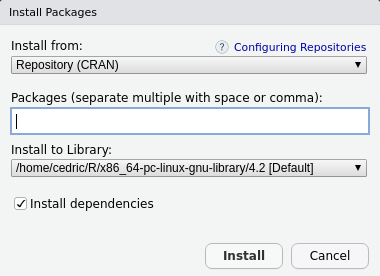
\includegraphics{~/Images/install_packages2.png}
\caption{Installer un package sous CRAN ou à partir d'une archive!}
\end{figure}

Une fois le package installé, vous pouvez charger le package à l'aide de la fonction \texttt{library()}ou en cochant la case devant le package dans la fenêtre \emph{Packages}.

\begin{figure}
\centering
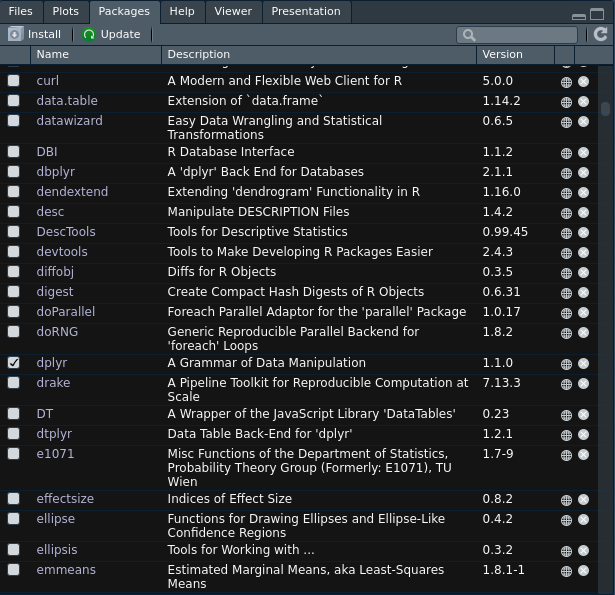
\includegraphics{~/Images/load_packages.png}
\caption{Charger un package comme dplyr!}
\end{figure}

Vous pouvez également utiliser la commande require() pour charger le package uniquement si le package n'est pas déjà chargé. Une fois le package chargé, vous pouvez utiliser les fonctions et les outils fournis par le package.\\
Le code ci-dessous permet d'installer et charger le package plyr.

\begin{Shaded}
\begin{Highlighting}[]
\FunctionTok{install.packages}\NormalTok{(}\StringTok{"plyr"}\NormalTok{)}
\end{Highlighting}
\end{Shaded}

\begin{verbatim}
## Error in install.packages : Updating loaded packages
\end{verbatim}

\begin{Shaded}
\begin{Highlighting}[]
\FunctionTok{library}\NormalTok{(plyr)}
\end{Highlighting}
\end{Shaded}

La fonction \texttt{update.packages()} permet de mettre à jour automatiquement les versions de tous les packages installés. Sous RStudio, on utilisera l'option Update de l'onglet \emph{Packages} qui permet de sélectionner les packages à mettre à jour.

\hypertarget{manipulation-des-donnuxe9es-sous-r}{%
\section{Manipulation des données sous R}\label{manipulation-des-donnuxe9es-sous-r}}

\hypertarget{importer-un-jeu-de-donnuxe9es-sous-r}{%
\subsection{importer un jeu de données sous R}\label{importer-un-jeu-de-donnuxe9es-sous-r}}

Il existe plusieurs façons d'importer des jeux de données sous R. La méthode la plus courante est d'utiliser la fonction \texttt{read.csv()} ou \texttt{read.table()} pour importer des \emph{fichiers CSV} ou des \emph{fichiers texte tabulés}. Ces fonctions peuvent lire des fichiers locaux ou des fichiers à partir d'URL. Vous pouvez également utiliser la fonction \texttt{read.xlsx()} pour importer des \emph{fichiers Excel}. Les autres méthodes d'importation comprennent l'utilisation des packages R spécialisés pour importer des données à partir de \emph{bases de données, d'API Web et d'autres sources}.

\begin{quote}
read.csv(``chemin/vers/le/fichier.csv'', header = TRUE, sep = ``,'')
\end{quote}

La fonction ci-dessus prend un paramètre obligatoire qui est le nom de fichier externe en format texte. Il doit être fourni entre guillemets et peut inclure le chemin d'accès au fichier si celui-ci ne se trouve pas dans le répertoire de travail. On peut trouver d'autres paramètres optionnels, comme:

\begin{longtable}[]{@{}
  >{\raggedright\arraybackslash}p{(\columnwidth - 2\tabcolsep) * \real{0.5000}}
  >{\raggedright\arraybackslash}p{(\columnwidth - 2\tabcolsep) * \real{0.5000}}@{}}
\toprule()
\begin{minipage}[b]{\linewidth}\raggedright
Paramètre
\end{minipage} & \begin{minipage}[b]{\linewidth}\raggedright
Description
\end{minipage} \\
\midrule()
\endhead
header & Une valeur logique (T/F) qui indique si la première ligne contient les noms des colonnes, sinon elles s'appelleront V1, V2\ldots{} header=F par défaut. \\
sep & Le caractère séparant les colonnes du tableau. Par défaut c'est l'espace. Si votre fichier est délimité par des tabulations, utilisez sep= ``\t". \\
dec & Le caractère utilisé comme séparateur decimal, par défaut c'est le ``.'' mais vous pouvez définir la ``,'' si votre tableau est au format français. \\
row.names & Les noms des lignes. Cela peut être un vecteur de même longueur que le nombre de lignes du tableau, mais on utilise souvent le numéro d'une colonne (généralement la première) qui sert alors de label aux lignes et se trouve exclue du tableau. \\
\bottomrule()
\end{longtable}

Il existe plusieurs fonctions utiles pour inspecter un tableau de données sous R:

\begin{quote}
\begin{itemize}
\tightlist
\item
  \texttt{str()} peut être utilisée pour afficher la structure d'un tableau de données.
\item
  \texttt{summary()} peut être utilisée pour afficher des statistiques descriptives sur chaque variable.
\item
  \texttt{head()} et \texttt{tail()} peuvent être utilisées pour afficher les premières et dernières lignes d'un tableau de données.
\item
  \texttt{dim()} peut être utilisée pour afficher le nombre de lignes et de colonnes dans un tableau de données.
\item
  \texttt{colnames()} peut être utilisée pour afficher les noms des colonnes.
\end{itemize}
\end{quote}

R comprend un certain nombre de \emph{jeux de données intégrés}. Ces jeux de données sont généralement organisés sous \textbf{forme de tableaux ou de matrices} et peuvent contenir des \emph{informations sur les variables, les observations et les caractéristiques de chaque observation}. Les jeux de données intégrés à R incluent des données sur le comportement des animaux, le climat, la géographie, la finance et bien plus encore. Les données peuvent être analysées et manipulées à l'aide de fonctions intégrées à R. Il existe également de nombreux packages tiers qui offrent des fonctionnalités supplémentaires pour traiter les données.\\
On utilise ici le jeu de données \textbf{ChickWeight} qui donne les résultats d'une expérimentation visant à comparer le poids des poussins à différents âges en fonction du régime alimentaire reçu.

\begin{Shaded}
\begin{Highlighting}[]
\CommentTok{\# Charger le jeu de données}
\FunctionTok{data}\NormalTok{(}\StringTok{"ChickWeight"}\NormalTok{)}

\CommentTok{\# Afficher les premières lignes du jeu de données}
\FunctionTok{head}\NormalTok{(ChickWeight)}
\end{Highlighting}
\end{Shaded}

\begin{verbatim}
##   weight Time Chick Diet
## 1     42    0     1    1
## 2     51    2     1    1
## 3     59    4     1    1
## 4     64    6     1    1
## 5     76    8     1    1
## 6     93   10     1    1
\end{verbatim}

\begin{Shaded}
\begin{Highlighting}[]
\CommentTok{\# Afficher les informations sur les variables du jeu de données}
\FunctionTok{str}\NormalTok{(ChickWeight)}
\end{Highlighting}
\end{Shaded}

\begin{verbatim}
## Classes 'nfnGroupedData', 'nfGroupedData', 'groupedData' and 'data.frame':   578 obs. of  4 variables:
##  $ weight: num  42 51 59 64 76 93 106 125 149 171 ...
##  $ Time  : num  0 2 4 6 8 10 12 14 16 18 ...
##  $ Chick : Ord.factor w/ 50 levels "18"<"16"<"15"<..: 15 15 15 15 15 15 15 15 15 15 ...
##  $ Diet  : Factor w/ 4 levels "1","2","3","4": 1 1 1 1 1 1 1 1 1 1 ...
##  - attr(*, "formula")=Class 'formula'  language weight ~ Time | Chick
##   .. ..- attr(*, ".Environment")=<environment: R_EmptyEnv> 
##  - attr(*, "outer")=Class 'formula'  language ~Diet
##   .. ..- attr(*, ".Environment")=<environment: R_EmptyEnv> 
##  - attr(*, "labels")=List of 2
##   ..$ x: chr "Time"
##   ..$ y: chr "Body weight"
##  - attr(*, "units")=List of 2
##   ..$ x: chr "(days)"
##   ..$ y: chr "(gm)"
\end{verbatim}

\begin{Shaded}
\begin{Highlighting}[]
\CommentTok{\# Afficher une description statistique des variables du jeu de données}
\FunctionTok{summary}\NormalTok{(ChickWeight)}
\end{Highlighting}
\end{Shaded}

\begin{verbatim}
##      weight           Time           Chick     Diet   
##  Min.   : 35.0   Min.   : 0.00   13     : 12   1:220  
##  1st Qu.: 63.0   1st Qu.: 4.00   9      : 12   2:120  
##  Median :103.0   Median :10.00   20     : 12   3:120  
##  Mean   :121.8   Mean   :10.72   10     : 12   4:118  
##  3rd Qu.:163.8   3rd Qu.:16.00   17     : 12          
##  Max.   :373.0   Max.   :21.00   19     : 12          
##                                  (Other):506
\end{verbatim}

\hypertarget{exporter-un-jeu-de-donnuxe9es-sous-r}{%
\subsection{Exporter un jeu de données sous R}\label{exporter-un-jeu-de-donnuxe9es-sous-r}}

Vous pouvez exporter les jeux de données sous R vers d'autres formats de fichier, tels que \emph{CSV, TXT ou XLS}. Vous pouvez également exporter des jeux de données vers des formats spécifiques à des applications, tels que SPSS, SAS ou Stata. La fonction \texttt{write.csv()} est l'une des fonctions les plus couramment utilisées pour exporter des jeux de données sous R. Elle permet d'exporter des jeux de données vers un fichier CSV.

\begin{quote}
write.csv(data, file = ``data.csv'', row.names = FALSE, na = ``\,``)
\end{quote}

\begin{itemize}
\tightlist
\item
  La fonction ci-dessus prend le jeu de données \emph{data} à exporter.\\
\item
  Le paramètre \emph{file} sauve le jeu de données data sous ``data.csv''.\\
\item
  Le paramètre \emph{row.names} indique si les noms de lignes sont incluses ou non dans le fichier csv.\\
\item
  Le paramètre \emph{na} indique la valeur à utiliser pour les valeurs manquantes.
\end{itemize}

\textbf{Exercice 1:}

\begin{enumerate}
\def\labelenumi{\arabic{enumi}.}
\tightlist
\item
  Charger le jeu de données prédéfini \textbf{mtcars} en utilisant la fonction \texttt{data()} de R. Vous pouvez utiliser l'aide R associée à mtcars pour en savoir plus. Explorer le data.frame mtcars en utilisant les fonctions \texttt{str()}, \texttt{head()}, \texttt{summary()} et \texttt{dim()}.
\item
  Exporter le data.frame mtcars en format texte dans le répertoire de travail sous le nom de \textbf{mtcars.csv}. Ensuite, vérifier la présence du fichier \emph{mtcars.csv} dans le répertoire de travail et l'ouvrir avec un tableur.
\item
  Dans ce tableur, ajouter une douzième colonne intitulée \textbf{mpg\_level} contenant les valeurs \emph{``faible''} pour les voitures ayant une consommation en miles par gallon (mpg) inférieure à 20, \emph{``moyenne''} pour celles ayant une consommation comprise entre 20 et 30, et \emph{``élevée''} pour celles ayant une consommation supérieure à 30. Enregistrer ce fichier au format texte délimité par des \emph{tabulations} sous le nom \textbf{mtcars2.csv}.
\item
  Puis retourner sous R et importer ce fichier de données dans un nouveau data.frame appelé \textbf{mtcars\_new}. Vérifiez son contenu sous R avec \texttt{dim()}, \texttt{head()}, etc. On voit que mtcars n'a plus comme nom de ligne, les marques de voitures, mais des chiffres au format caractères.\\
  Essayez donc d'attribuer les noms de lignes aux marques de voitures et supprimer la colonne X.
\end{enumerate}

\hypertarget{statistiques-descriptives-avec-r}{%
\section{Statistiques descriptives avec R}\label{statistiques-descriptives-avec-r}}

Les statistiques descriptives sont un ensemble de méthodes utilisées pour analyser et interpréter des données. Avec R, vous pouvez facilement réaliser des analyses statistiques descriptives, telles que les \textbf{moyennes}, les \textbf{écarts-types}, les \textbf{quantiles} et bien plus encore. Vous pouvez également créer des graphiques et des tableaux pour mieux comprendre et interpréter vos données.

\hypertarget{muxe9dianes-et-quantiles}{%
\subsection{Médianes et quantiles}\label{muxe9dianes-et-quantiles}}

Sous R, il est possible de calculer la médiane et les quantiles d'un vecteur ou d'une colonne d'un data.frame à l'aide de fonctions de base. Voici quelques explications:

\begin{itemize}
\tightlist
\item
  La \textbf{médiane} est la valeur centrale d'un ensemble de données triées par ordre croissant ou décroissant. Elle divise l'ensemble en deux parties égales. En R, la fonction \texttt{median()} permet de calculer la médiane d'un vecteur ou d'une colonne d'un data.frame.
\end{itemize}

\begin{Shaded}
\begin{Highlighting}[]
\CommentTok{\#Création d\textquotesingle{}un vecteur}
\NormalTok{x }\OtherTok{\textless{}{-}} \FunctionTok{c}\NormalTok{(}\DecValTok{3}\NormalTok{, }\DecValTok{5}\NormalTok{, }\DecValTok{6}\NormalTok{, }\DecValTok{9}\NormalTok{, }\DecValTok{10}\NormalTok{, }\DecValTok{12}\NormalTok{, }\DecValTok{15}\NormalTok{, }\DecValTok{18}\NormalTok{, }\DecValTok{19}\NormalTok{, }\DecValTok{20}\NormalTok{)}

\CommentTok{\# Calcul de la médiane}
\FunctionTok{median}\NormalTok{(x)}
\end{Highlighting}
\end{Shaded}

\begin{verbatim}
## [1] 11
\end{verbatim}

Le résultat sera 11, la valeur centrale du vecteur trié par ordre croissant.

\begin{itemize}
\tightlist
\item
  Les \textbf{quantiles} sont des valeurs qui divisent l'ensemble de données en parts égales. Par exemple, le premier quartile (Q1) est la valeur qui divise les données en deux parties égales, la première moitié ayant des valeurs inférieures ou égales à Q1, et la seconde moitié ayant des valeurs supérieures ou égales à Q1. En R, la fonction \texttt{quantile()} permet de calculer les quantiles d'un vecteur ou d'une colonne d'un data.frame.
\end{itemize}

\begin{Shaded}
\begin{Highlighting}[]
\CommentTok{\# Calcul des quartiles d\textquotesingle{}un vecteur}
\FunctionTok{quantile}\NormalTok{(x, }\AttributeTok{probs =} \FunctionTok{c}\NormalTok{(}\FloatTok{0.25}\NormalTok{, }\FloatTok{0.5}\NormalTok{, }\FloatTok{0.75}\NormalTok{))}
\end{Highlighting}
\end{Shaded}

\begin{verbatim}
##   25%   50%   75% 
##  6.75 11.00 17.25
\end{verbatim}

Ce qui signifie que le premier quartile est 6.75, la médiane est 11, et le troisième quartile est 17.25.

\hypertarget{la-moyenne-et-la-somme}{%
\subsection{La moyenne et la somme}\label{la-moyenne-et-la-somme}}

Sous R, la moyenne et la somme sont deux concepts importants en statistiques et en programmation. Voici comment les calculer :

\begin{itemize}
\tightlist
\item
  La \textbf{moyenne} est la somme de tous les éléments d'un ensemble de données, divisée par le nombre total d'éléments. En R, vous pouvez calculer la moyenne à l'aide de la fonction \texttt{mean()}.
\end{itemize}

\begin{Shaded}
\begin{Highlighting}[]
\CommentTok{\# Créer un vecteur de données}
\NormalTok{x }\OtherTok{\textless{}{-}} \FunctionTok{c}\NormalTok{(}\DecValTok{1}\NormalTok{, }\DecValTok{2}\NormalTok{, }\DecValTok{3}\NormalTok{, }\DecValTok{4}\NormalTok{, }\DecValTok{5}\NormalTok{)}

\CommentTok{\# Calculer la moyenne}
\FunctionTok{mean}\NormalTok{(x)}
\end{Highlighting}
\end{Shaded}

\begin{verbatim}
## [1] 3
\end{verbatim}

Dans cet exemple, la moyenne de 1, 2, 3, 4 et 5 est 3.

\begin{itemize}
\tightlist
\item
  La \textbf{somme} est la valeur totale de tous les éléments d'un ensemble de données. En R, vous pouvez calculer la somme à l'aide de la fonction \texttt{sum()}.
\end{itemize}

\begin{Shaded}
\begin{Highlighting}[]
\CommentTok{\# Créer un vecteur de données}
\NormalTok{x }\OtherTok{\textless{}{-}} \FunctionTok{c}\NormalTok{(}\DecValTok{1}\NormalTok{, }\DecValTok{2}\NormalTok{, }\DecValTok{3}\NormalTok{, }\DecValTok{4}\NormalTok{, }\DecValTok{5}\NormalTok{)}

\CommentTok{\# Calculer la somme}
\FunctionTok{sum}\NormalTok{(x)}
\end{Highlighting}
\end{Shaded}

\begin{verbatim}
## [1] 15
\end{verbatim}

Dans cet exemple, la somme de 1, 2, 3, 4 et 5 est 15.

\hypertarget{la-variance-et-luxe9cart-type}{%
\subsection{La variance et l'écart-type}\label{la-variance-et-luxe9cart-type}}

La variance et l'écart-type sont deux mesures importantes de la \textbf{dispersion des données}.

\begin{itemize}
\tightlist
\item
  La \textbf{variance} est une mesure de la dispersion des données par \emph{rapport à leur moyenne} (moyenne des carrés des écarts entre chaque valeur de x
  et la moyenne). En R, vous pouvez calculer la variance à l'aide de la fonction \texttt{var()}.
\end{itemize}

\begin{Shaded}
\begin{Highlighting}[]
\CommentTok{\# Créer un vecteur de données}
\NormalTok{x }\OtherTok{\textless{}{-}} \FunctionTok{c}\NormalTok{(}\DecValTok{1}\NormalTok{, }\DecValTok{2}\NormalTok{, }\DecValTok{3}\NormalTok{, }\DecValTok{4}\NormalTok{, }\DecValTok{5}\NormalTok{)}

\CommentTok{\# Calculer la variance}
\FunctionTok{var}\NormalTok{(x)}
\end{Highlighting}
\end{Shaded}

\begin{verbatim}
## [1] 2.5
\end{verbatim}

Dans cet exemple, la variance de 1, 2, 3, 4 et 5 est 2,5.

\begin{itemize}
\tightlist
\item
  L'écart-type est une mesure de la dispersion des données qui est \emph{la racine carrée de la variance}, qui a l'avantage de
  s'exprimer dans la même unité que la moyenne et que les données. En R, vous pouvez calculer l'écart-type à l'aide de la fonction \texttt{sd()}.
\end{itemize}

\begin{Shaded}
\begin{Highlighting}[]
\CommentTok{\# Créer un vecteur de données}
\NormalTok{x }\OtherTok{\textless{}{-}} \FunctionTok{c}\NormalTok{(}\DecValTok{1}\NormalTok{, }\DecValTok{2}\NormalTok{, }\DecValTok{3}\NormalTok{, }\DecValTok{4}\NormalTok{, }\DecValTok{5}\NormalTok{)}

\CommentTok{\# Calculer l\textquotesingle{}écart{-}type}
\FunctionTok{sd}\NormalTok{(x)}
\end{Highlighting}
\end{Shaded}

\begin{verbatim}
## [1] 1.581139
\end{verbatim}

Dans cet exemple, l'écart-type de 1, 2, 3, 4 et 5 est 1,581139.

\begin{quote}
Il est important de noter que ces fonctions fonctionnent également avec des matrices et des tableaux, où elles effectueront le calcul par colonne par défaut. Vous pouvez également spécifier l'argument ``na.rm'' pour exclure les valeurs manquantes.
\end{quote}

\textbf{Exercices 2:}

Sur le jeu de données ``ChickWeight'', utilisez les fonctions que l'on
vient de voir pour faire une description statistique de la colonne weight.

\hypertarget{ruxe9gression-linuxe9aire}{%
\section{Régression linéaire}\label{ruxe9gression-linuxe9aire}}

La régression linéaire est une méthode statistique utilisée pour modéliser la \textbf{relation entre une variable dépendante et une ou plusieurs variables indépendantes}. Sous R, il est possible d'effectuer une régression linéaire à l'aide de la fonction \texttt{lm()}.\\
La régression linéaire simple (une seule variable explicative) s'écrit:

\begin{quote}
lm(y\textasciitilde x)
\end{quote}

Dans l'exemple suivant, on va tester la relation entre le poids et lâge des poussins.

\begin{Shaded}
\begin{Highlighting}[]
\CommentTok{\#chargement du jeu de données}
\FunctionTok{data}\NormalTok{(}\StringTok{"ChickWeight"}\NormalTok{)}

\NormalTok{m }\OtherTok{\textless{}{-}} \FunctionTok{lm}\NormalTok{(weight}\SpecialCharTok{\textasciitilde{}}\NormalTok{Time, }\AttributeTok{data =}\NormalTok{ ChickWeight)}
\FunctionTok{summary}\NormalTok{(m)}
\end{Highlighting}
\end{Shaded}

\begin{verbatim}
## 
## Call:
## lm(formula = weight ~ Time, data = ChickWeight)
## 
## Residuals:
##      Min       1Q   Median       3Q      Max 
## -138.331  -14.536    0.926   13.533  160.669 
## 
## Coefficients:
##             Estimate Std. Error t value Pr(>|t|)    
## (Intercept)  27.4674     3.0365   9.046   <2e-16 ***
## Time          8.8030     0.2397  36.725   <2e-16 ***
## ---
## Signif. codes:  0 '***' 0.001 '**' 0.01 '*' 0.05 '.' 0.1 ' ' 1
## 
## Residual standard error: 38.91 on 576 degrees of freedom
## Multiple R-squared:  0.7007, Adjusted R-squared:  0.7002 
## F-statistic:  1349 on 1 and 576 DF,  p-value: < 2.2e-16
\end{verbatim}

Ce résultat concerne un modèle de régression linéaire simple pour prédire le poids des poussins en fonction de leur âge. Voici comment interpréter les différents éléments :

\begin{quote}
\begin{itemize}
\tightlist
\item
  Call : Cette ligne indique la formule de régression utilisée, qui est ``weight \textasciitilde{} Time'' et le nom du data.frame utilisé, qui est ``ChickWeight''.
\item
  Coefficients : Cette section présente les coefficients de la régression. L'intercept (l'ordonnée à l'origine) est de 27,4674 et la pente pour la variable ``Time'' est de 8,8030. Cela signifie que pour chaque unité de temps supplémentaire (jours), le poids des poussins augmente en moyenne de 8,8030.
\item
  Pr(\textgreater\textbar t\textbar) : Cette colonne donne la p-value pour chaque coefficient. Les p-values très faibles (\textless{} 0,001) indiquent que les coefficients sont significatifs et que la probabilité d'obtenir une telle valeur de t par hasard est très faible.
\item
  Residual standard error : C'est une estimation de l'écart-type des résidus. Cela mesure la variabilité non expliquée du modèle. Dans ce cas, l'écart-type est de 38,91.
\item
  Multiple R-squared : C'est le coefficient de détermination qui mesure la proportion de la variance totale expliquée par le modèle. Ici, le R² est de 0,7007, ce qui indique que le modèle explique 70,07 \% de la variance totale des données.
\item
  F-statistic : Il s'agit d'un test statistique global de la significativité du modèle. Dans ce cas, le F-statistic est de 1349 avec 1 et 576 degrés de liberté, ce qui est très significatif.
\item
  p-value : C'est la p-value associée au test F et indique la probabilité d'obtenir une telle valeur de F par hasard. La p-value est très faible (\textless{} 2,2e-16), ce qui indique que le modèle est très significatif.
\end{itemize}
\end{quote}

\textbf{En résumé, ce modèle de régression linéaire simple montre qu'il existe une relation positive significative entre le poids des poussins et leur âge. Le modèle explique environ 70 \% de la variance totale des données et est très significatif.}

Ajoutons maintenant le régime alimentaire des poussins en compte. Voyons maintenant l'effet de l'âge et du régime alimentaire sur le poids des poussins.
Le modèle devient:

\begin{Shaded}
\begin{Highlighting}[]
\CommentTok{\#chargement du jeu de données}
\FunctionTok{data}\NormalTok{(}\StringTok{"ChickWeight"}\NormalTok{)}

\NormalTok{m }\OtherTok{\textless{}{-}} \FunctionTok{lm}\NormalTok{(weight}\SpecialCharTok{\textasciitilde{}}\NormalTok{Time}\SpecialCharTok{*}\NormalTok{Diet, }\AttributeTok{data =}\NormalTok{ ChickWeight)}
\FunctionTok{summary}\NormalTok{(m)}
\end{Highlighting}
\end{Shaded}

\begin{verbatim}
## 
## Call:
## lm(formula = weight ~ Time * Diet, data = ChickWeight)
## 
## Residuals:
##      Min       1Q   Median       3Q      Max 
## -135.425  -13.757   -1.311   11.069  130.391 
## 
## Coefficients:
##             Estimate Std. Error t value Pr(>|t|)    
## (Intercept)  30.9310     4.2468   7.283 1.09e-12 ***
## Time          6.8418     0.3408  20.076  < 2e-16 ***
## Diet2        -2.2974     7.2672  -0.316  0.75202    
## Diet3       -12.6807     7.2672  -1.745  0.08154 .  
## Diet4        -0.1389     7.2865  -0.019  0.98480    
## Time:Diet2    1.7673     0.5717   3.092  0.00209 ** 
## Time:Diet3    4.5811     0.5717   8.014 6.33e-15 ***
## Time:Diet4    2.8726     0.5781   4.969 8.92e-07 ***
## ---
## Signif. codes:  0 '***' 0.001 '**' 0.01 '*' 0.05 '.' 0.1 ' ' 1
## 
## Residual standard error: 34.07 on 570 degrees of freedom
## Multiple R-squared:  0.773,  Adjusted R-squared:  0.7702 
## F-statistic: 277.3 on 7 and 570 DF,  p-value: < 2.2e-16
\end{verbatim}

Cette régression linéaire est un modèle plus complexe que le précédent car il inclut non seulement l'effet de l'âge sur le poids des poussins, mais aussi l'effet du régime alimentaire sur leur poids. De plus, il inclut également une \textbf{interaction entre l'âge et la diète}, ce qui permet d'explorer si l'effet de l'âge sur le poids varie selon la diète.

Voici comment interpréter les résultats :

\begin{quote}
\begin{itemize}
\tightlist
\item
  Pour l'intercept, Diet1 est pris comme référence. Si nous considérons que la référence (Diet1) a un poids initial moyen de 30.9310g, le coefficient pour Diet2 indique que les poussins ont un poids initial de 28.6336g (30.9310 - 2.2974) lorsqu'ils ont commencé l'expérience.
\item
  Le coefficient pour Time indique que, toutes choses égales par ailleurs, le poids des poussins augmente de 6.8418g chaque jour qui passe.
\item
  Les coefficients pour Time:Diet2, Time:Diet3, et Time:Diet4 indiquent l'effet de l'interaction entre le temps et la diète respective sur le poids des poussins. Par exemple, le coefficient pour Time:Diet3 indique que l'effet, de chaque jour supplémentaire sur le poids des poussins, est amplifié de 4.5811g pour les poussins qui reçoivent Diet3, comparé à ceux qui reçoivent la diète de référence.
\item
  La valeur de l'erreur standard résiduelle (Residual standard error) est de 34.07, ce qui indique l'erreur standard moyenne dans les prévisions du poids des poussins que le modèle ne peut pas expliquer.
\item
  Le R-carré multiple (Multiple R-squared) indique la proportion de la variance totale qui est expliquée par le modèle, et est égal à 0.773. Cela signifie que le modèle explique environ 77,3\% de la variation totale des données.
\item
  L'ajustement du R-carré (Adjusted R-squared) est égal à 0.7702. Cela signifie que le modèle ajusté explique environ 77,0\% de la variation des données.
\item
  Le test F, avec une statistique de test de 277.3 et une p-value très faible, indique que le modèle dans son ensemble est significatif.
\end{itemize}
\end{quote}

\textbf{En résumé, ce modèle de régression linéaire montre qu'il existe une relation significative à la fois entre le poids des poussins, leur âge et le régime alimentaire reçu. Le modèle explique environ 77 \% de la variance totale des données et est très significatif.}

\textbf{Exercice 3:}

Le jeu de données \textbf{iris} intégré dans R contient des mesures sur différentes espèces d'iris. Nous allons utiliser la longueur du pétale (Petal.Length) pour prédire la largeur du pétale (Petal.Width).

\begin{enumerate}
\def\labelenumi{\arabic{enumi}.}
\tightlist
\item
  Charger le jeu de données ``iris'' en utilisant la fonction \texttt{data()}.
\item
  Examiner les données en utilisant la fonction \texttt{head()} et \texttt{summary()}.
\item
  Créer un graphique de dispersion de Petal.Length vs Petal.Width en utilisant la fonction \texttt{plot()}.
\item
  Ajuster un modèle de régression linéaire simple pour prédire Petal.Width à partir de Petal.Length.
\item
  Résumer les résultats de la régression en utilisant la fonction \texttt{summary()}.
\item
  Utiliser le modèle pour faire une prédiction de la largeur du pétale pour une fleur avec une longueur de pétale de 6 cm.
\item
  Tracer la ligne de régression sur le graphique de dispersion en utilisant la fonction \texttt{abline()}.
\end{enumerate}

\hypertarget{les-graphiques-avec-r}{%
\section{Les graphiques avec R}\label{les-graphiques-avec-r}}

\hypertarget{gestion-des-graphiques-sous-rstudio}{%
\subsection{Gestion des graphiques sous RStudio}\label{gestion-des-graphiques-sous-rstudio}}

RStudio possède une fenêtre graphique intégrée où les graphiques peuvent être affichés. Cette fenêtre peut être agrandie, réduite ou mise en plein écran, et permet également de zoomer sur des parties spécifiques du graphique. Cette fenêtre permet également d'enregistrer le graphique dans différents formats de fichiers, tels que PNG, PDF, JPEG, SVG, etc.

\begin{figure}
\centering
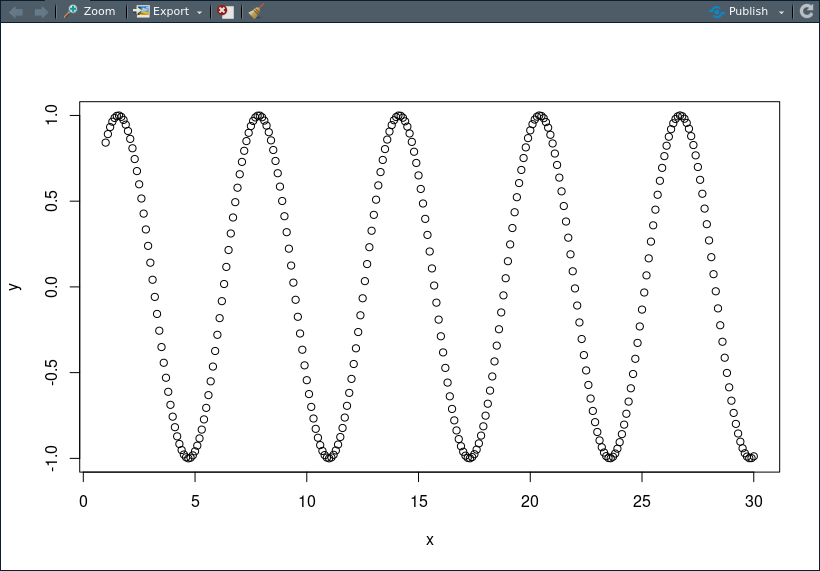
\includegraphics{~/Images/rstudio_graph.png}
\caption{Affichage d'un graphique sous RStudio!}
\end{figure}

On peut aussi, avant l'appel à la fonction graphique, ouvrir une nouvelle fenêtre graphique avec la fonction \texttt{x11()} qui fonctionne sur Linux et Windows ou son équivalent \texttt{windows()} (Windows uniquement), ou encore \texttt{quartz()} sous MacOS. Le graphique s'affichera toujours dans la dernière fenêtre graphique ouverte qui devient le périphérique (device) actif.
On peut également ouvrir directement un fichier graphique avec la fonction \texttt{pdf()}, ou \texttt{jpeg()}\ldots{} Taper \textbf{?Devices} pour connaître les différents périphériques utilisables.

Dans RStudio, la fonction \texttt{dev.new()} ouvre un nouveau périphérique graphique. La fonction \texttt{dev.set()} permet de sélectionner un périphérique graphique existant. Elle peut être utilisée pour basculer entre les périphériques graphiques ouverts. Par exemple, si vous avez deux périphériques graphiques ouverts, vous pouvez utiliser dev.set(1) pour sélectionner le premier périphérique et dev.set(2) pour sélectionner le deuxième périphérique. La fonction \texttt{dev.off()} ferme le périphérique graphique actif. Cela peut être utile si vous avez plusieurs fenêtres graphiques ouvertes et que vous souhaitez en fermer une.

Il est également possible de sauvegarder les graphiques créés dans RStudio en utilisant la fonction \texttt{dev.copy()}. Cette fonction copie le graphique actif vers un périphérique spécifié, tel qu'un fichier PDF ou une image PNG. Par exemple, dev.copy(pdf, ``myplot.pdf'') copiera le graphique actif dans un fichier PDF nommé ``plot1.pdf''.

\begin{Shaded}
\begin{Highlighting}[]
\FunctionTok{X11}\NormalTok{()   }
\NormalTok{x }\OtherTok{\textless{}{-}} \FunctionTok{seq}\NormalTok{(}\DecValTok{1}\NormalTok{,}\DecValTok{30}\NormalTok{,}\FloatTok{0.1}\NormalTok{)}
\NormalTok{y }\OtherTok{\textless{}{-}} \FunctionTok{sin}\NormalTok{(x)}
\FunctionTok{plot}\NormalTok{(x,y, }\AttributeTok{type=}\StringTok{"p"}\NormalTok{)}
\FunctionTok{dev.copy}\NormalTok{(pdf, }\StringTok{"plot1.pdf"}\NormalTok{)}
\FunctionTok{dev.off}\NormalTok{()}
\end{Highlighting}
\end{Shaded}

Enfin, il est possible de personnaliser la sortie graphique en modifiant les \textbf{options} de périphériques graphiques. Par exemple, vous pouvez spécifier la taille de la fenêtre graphique avec \emph{options(``dev.size'' = c(7, 5))} pour une fenêtre de 7 pouces de large et 5 pouces de haut. Vous pouvez également spécifier le type de périphérique graphique à utiliser par défaut avec options(``device'' = ``pdf'').

\hypertarget{quelques-fonctions-graphiques}{%
\subsection{Quelques fonctions graphiques}\label{quelques-fonctions-graphiques}}

\hypertarget{la-fonction-plot}{%
\subsubsection{La fonction plot()}\label{la-fonction-plot}}

La fonction \texttt{plot()} est une fonction de base de R qui permet de créer des graphiques. Elle est très versatile et permet de créer différents types de graphiques en fonction des arguments passés en entrée. Voici quelques exemples de graphiques que l'on peut créer avec la fonction plot():

\begin{enumerate}
\def\labelenumi{\arabic{enumi}.}
\item
  Graphique de dispersion (scatterplot):

  Un graphique de dispersion permet de visualiser la relation entre deux variables continues. On peut créer un tel graphique avec plot() en passant en entrée les valeurs de la première variable sur l'axe des x et les valeurs de la deuxième variable sur l'axe des y. Par exemple:

\begin{Shaded}
\begin{Highlighting}[]
\NormalTok{x }\OtherTok{\textless{}{-}} \FunctionTok{c}\NormalTok{(}\DecValTok{1}\NormalTok{, }\DecValTok{2}\NormalTok{, }\DecValTok{3}\NormalTok{, }\DecValTok{4}\NormalTok{, }\DecValTok{5}\NormalTok{)}
\NormalTok{y }\OtherTok{\textless{}{-}} \FunctionTok{c}\NormalTok{(}\DecValTok{2}\NormalTok{, }\DecValTok{4}\NormalTok{, }\DecValTok{6}\NormalTok{, }\DecValTok{8}\NormalTok{, }\DecValTok{10}\NormalTok{)}
\FunctionTok{plot}\NormalTok{(x, y)}
\end{Highlighting}
\end{Shaded}

  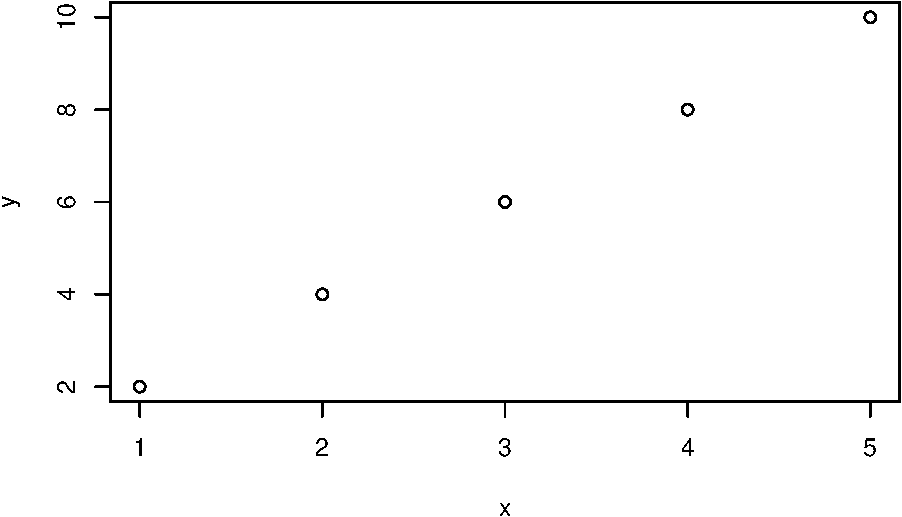
\includegraphics{_main_files/figure-latex/graph1-1.pdf}
\item
  Graphique de ligne:

  Un graphique de ligne permet de visualiser l'évolution d'une variable en fonction d'une autre variable (souvent une variable temporelle). On peut créer un tel graphique avec \texttt{plot()} en passant en entrée les valeurs de la première variable sur l'axe des x et les valeurs de la deuxième variable sur l'axe des y, et en spécifiant l'option \textbf{type=``l''}. Par exemple:

\begin{Shaded}
\begin{Highlighting}[]
\NormalTok{x }\OtherTok{\textless{}{-}} \FunctionTok{c}\NormalTok{(}\DecValTok{1}\NormalTok{, }\DecValTok{2}\NormalTok{, }\DecValTok{3}\NormalTok{, }\DecValTok{4}\NormalTok{, }\DecValTok{5}\NormalTok{)}
\NormalTok{y }\OtherTok{\textless{}{-}} \FunctionTok{c}\NormalTok{(}\DecValTok{2}\NormalTok{, }\DecValTok{4}\NormalTok{, }\DecValTok{6}\NormalTok{, }\DecValTok{8}\NormalTok{, }\DecValTok{10}\NormalTok{)}
\FunctionTok{plot}\NormalTok{(x, y, }\AttributeTok{type=}\StringTok{"l"}\NormalTok{)}
\end{Highlighting}
\end{Shaded}

  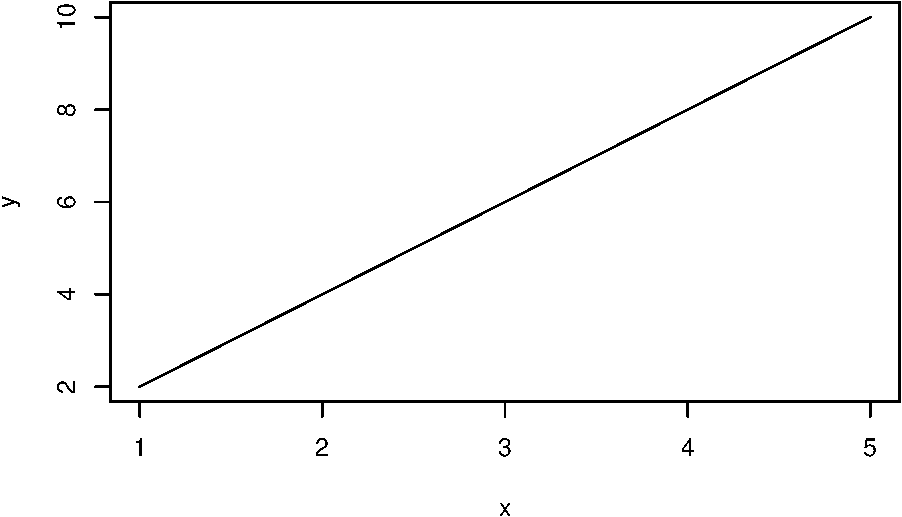
\includegraphics{_main_files/figure-latex/graph2-1.pdf}
\item
  Graphique en boîte (boxplot):

  Un graphique en boîte permet de visualiser la distribution d'une variable quantitative en fonction d'une variable qualitative. On peut créer un tel graphique avec \texttt{plot()} en passant en entrée la variable quantitative et la variable qualitative sous forme de facteur, et en spécifiant l'option type=``b''. Par exemple:

\begin{Shaded}
\begin{Highlighting}[]
\NormalTok{x }\OtherTok{\textless{}{-}} \FunctionTok{rnorm}\NormalTok{(}\DecValTok{100}\NormalTok{)}
\NormalTok{y }\OtherTok{\textless{}{-}} \FunctionTok{factor}\NormalTok{(}\FunctionTok{rep}\NormalTok{(}\FunctionTok{c}\NormalTok{(}\StringTok{"A"}\NormalTok{, }\StringTok{"B"}\NormalTok{), }\AttributeTok{each=}\DecValTok{50}\NormalTok{))}
\FunctionTok{plot}\NormalTok{(y, x, }\AttributeTok{type=}\StringTok{"b"}\NormalTok{)}
\end{Highlighting}
\end{Shaded}

  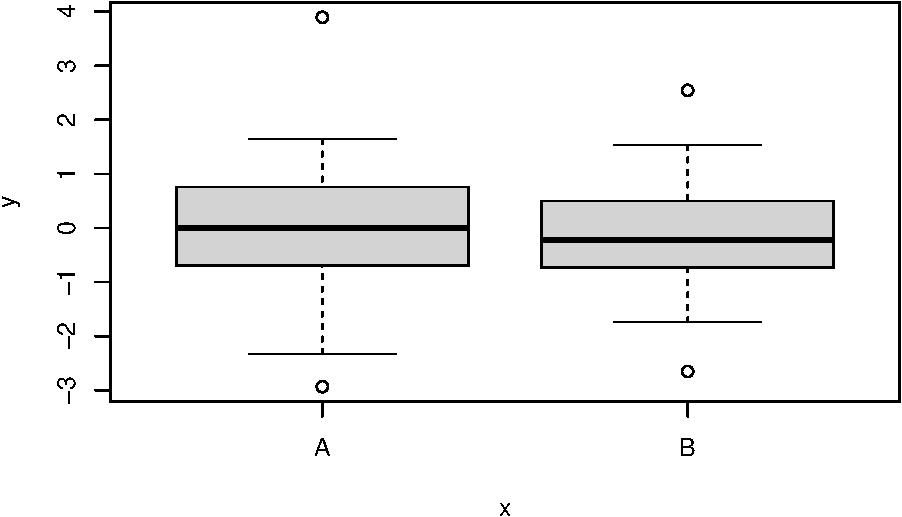
\includegraphics{_main_files/figure-latex/graph3-1.pdf}
\end{enumerate}

\hypertarget{la-fonction-pairs}{%
\subsubsection{La fonction pairs()}\label{la-fonction-pairs}}

La fonction \texttt{pairs()} permet de créer une \textbf{matrice de nuages de points pour visualiser les relations entre plusieurs variables} dans un ensemble de données. Elle prend en entrée une matrice ou un data frame contenant les variables à afficher et affiche une matrice de nuages de points où chaque case représente la relation entre deux variables.

Par exemple, supposons que nous avons un data.frame appelé \emph{iris} contenant les mesures de longueur et de largeur des pétales et des sépales pour trois espèces de fleurs. Pour afficher une matrice de nuages de points pour toutes les combinaisons possibles de ces quatre variables, nous pouvons utiliser la fonction \texttt{pairs()} comme suit:

\begin{Shaded}
\begin{Highlighting}[]
\CommentTok{\# Charger le jeu de données iris}
\FunctionTok{data}\NormalTok{(}\StringTok{"iris"}\NormalTok{)}

\CommentTok{\# Vecteur de couleurs pour chaque espèce}
\NormalTok{cols }\OtherTok{\textless{}{-}} \FunctionTok{c}\NormalTok{(}\StringTok{"red"}\NormalTok{, }\StringTok{"green"}\NormalTok{, }\StringTok{"blue"}\NormalTok{)}

\CommentTok{\# Utiliser la fonction pairs() avec l\textquotesingle{}argument col pour colorer chaque point en fonction de l\textquotesingle{}espèce correspondante}
\FunctionTok{pairs}\NormalTok{(iris[,}\DecValTok{1}\SpecialCharTok{:}\DecValTok{4}\NormalTok{], }\AttributeTok{col =}\NormalTok{ cols[iris}\SpecialCharTok{$}\NormalTok{Species])}
\end{Highlighting}
\end{Shaded}

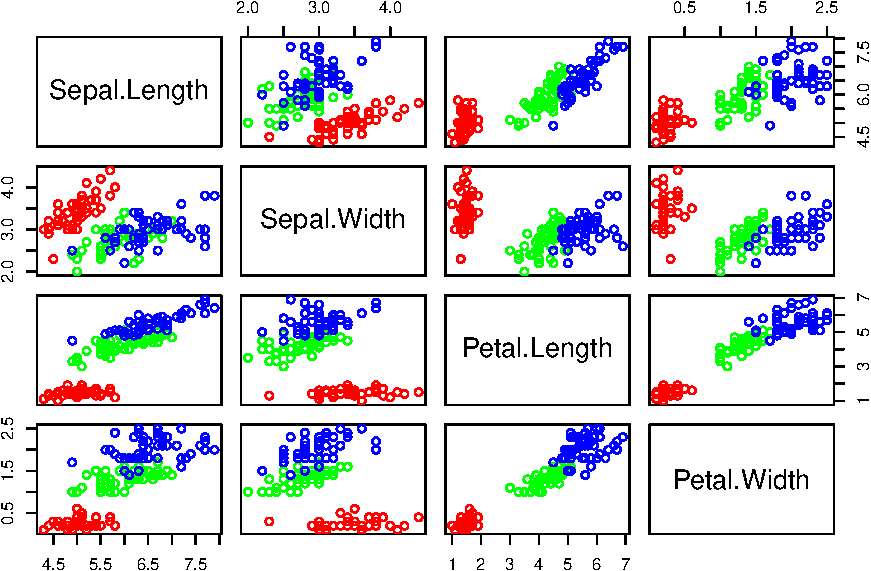
\includegraphics{_main_files/figure-latex/pairs-1.pdf}

Cela va afficher une matrice de 12 nuages de points, montrant les relations entre chaque paire de variables.\\
Ici, nous avons défini le vecteur cols pour contenir une couleur pour chaque espèce (red pour Setosa, green pour Versicolor et blue pour Virginica). Ensuite, nous avons utilisé l'argument col avec le vecteur de couleurs correspondant à chaque espèce (cols{[}iris\$Species{]}) pour colorer chaque point en fonction de l'espèce correspondante.

\hypertarget{la-fonction-pie}{%
\subsubsection{La fonction pie()}\label{la-fonction-pie}}

La fonction \texttt{pie} permet de représenter graphiquement des \textbf{proportions} dans un graphique circulaire.

\begin{Shaded}
\begin{Highlighting}[]
\NormalTok{x }\OtherTok{\textless{}{-}} \FunctionTok{c}\NormalTok{(}\FloatTok{0.2}\NormalTok{, }\FloatTok{0.3}\NormalTok{, }\FloatTok{0.1}\NormalTok{, }\FloatTok{0.4}\NormalTok{)}
\FunctionTok{pie}\NormalTok{(x)}
\end{Highlighting}
\end{Shaded}

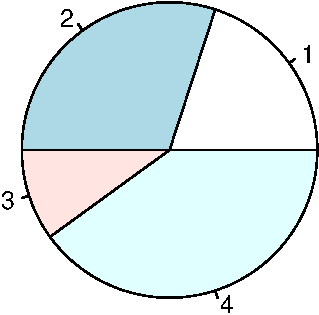
\includegraphics{_main_files/figure-latex/pie-1.pdf}

Le graphique qui en résulte présente un cercle divisé en quatre sections représentant chacune une proportion de l'ensemble.

\hypertarget{la-fonction-hist}{%
\subsubsection{La fonction hist()}\label{la-fonction-hist}}

La fonction \texttt{hist()} en R est utilisée pour créer un \textbf{histogramme}, qui est un type de graphique qui représente la distribution des valeurs numériques d'un vecteur. L'histogramme est un graphique en barres, où chaque barre représente une plage de valeurs, appelée \emph{bin ou classe}, et la hauteur de la barre représente le nombre de valeurs dans cette plage.

La fonction \texttt{hist()} prend en entrée un vecteur de données numériques et peut également accepter des arguments optionnels pour personnaliser le graphique, tels que le nombre de classes (bins) souhaité, les couleurs des barres, la couleur de fond, les étiquettes des axes, etc.

Voici un exemple d'utilisation de la fonction ``hist()'' pour créer un histogramme à partir d'un vecteur de données numériques ``x'':

\begin{Shaded}
\begin{Highlighting}[]
\CommentTok{\# Créer un vecteur de données}
\NormalTok{x }\OtherTok{\textless{}{-}} \FunctionTok{c}\NormalTok{(}\DecValTok{3}\NormalTok{, }\DecValTok{5}\NormalTok{, }\DecValTok{6}\NormalTok{, }\DecValTok{7}\NormalTok{, }\DecValTok{8}\NormalTok{, }\DecValTok{9}\NormalTok{, }\DecValTok{9}\NormalTok{, }\DecValTok{10}\NormalTok{, }\DecValTok{11}\NormalTok{, }\DecValTok{12}\NormalTok{, }\DecValTok{14}\NormalTok{, }\DecValTok{15}\NormalTok{, }\DecValTok{16}\NormalTok{, }\DecValTok{17}\NormalTok{, }\DecValTok{18}\NormalTok{, }\DecValTok{19}\NormalTok{, }\DecValTok{20}\NormalTok{)}

\CommentTok{\# Créer un histogramme avec 5 classes}
\FunctionTok{hist}\NormalTok{(x, }\AttributeTok{breaks =} \DecValTok{5}\NormalTok{, }\AttributeTok{main =} \StringTok{"Histogramme de x"}\NormalTok{, }\AttributeTok{xlab =} \StringTok{"Valeur de x"}\NormalTok{, }\AttributeTok{ylab =} \StringTok{"Fréquence"}\NormalTok{)}
\end{Highlighting}
\end{Shaded}

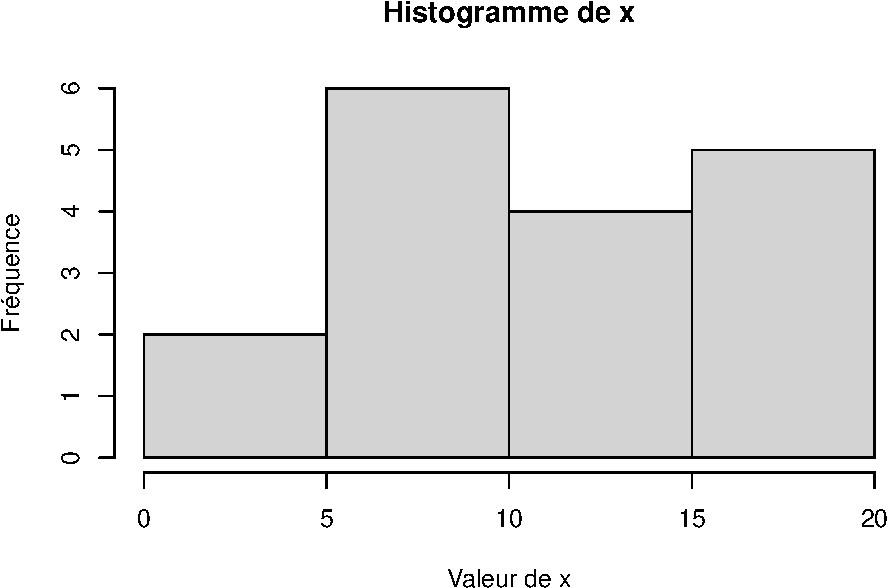
\includegraphics{_main_files/figure-latex/hist-1.pdf}

Dans cet exemple, la fonction \texttt{hist()} crée un histogramme avec 5 classes en utilisant le vecteur ``x'', et l'option \textbf{breaks}. Les options \textbf{main, xlab, ylab} sont utilisées pour ajouter des étiquettes de titre et d'axes au graphique.\\
A la place des fréquences, on peut afficher des \textbf{densités avec l'option freq=F}. On peut également ajouter une courbe de densité en utilisant la fonction \texttt{lines()} par-dessus la fonction de densité \texttt{density()}.

\begin{Shaded}
\begin{Highlighting}[]
\CommentTok{\# Créer un vecteur de données}
\NormalTok{x }\OtherTok{\textless{}{-}} \FunctionTok{c}\NormalTok{(}\DecValTok{3}\NormalTok{, }\DecValTok{5}\NormalTok{, }\DecValTok{6}\NormalTok{, }\DecValTok{7}\NormalTok{, }\DecValTok{8}\NormalTok{, }\DecValTok{9}\NormalTok{, }\DecValTok{9}\NormalTok{, }\DecValTok{10}\NormalTok{, }\DecValTok{11}\NormalTok{, }\DecValTok{12}\NormalTok{, }\DecValTok{14}\NormalTok{, }\DecValTok{15}\NormalTok{, }\DecValTok{16}\NormalTok{, }\DecValTok{17}\NormalTok{, }\DecValTok{18}\NormalTok{, }\DecValTok{19}\NormalTok{, }\DecValTok{20}\NormalTok{)}

\CommentTok{\# Créer un histogramme avec 5 classes}
\FunctionTok{hist}\NormalTok{(x, }\AttributeTok{breaks =} \DecValTok{5}\NormalTok{, }\AttributeTok{freq=}\NormalTok{F, }\AttributeTok{main =} \StringTok{"Histogramme de x"}\NormalTok{, }\AttributeTok{ylab =} \StringTok{"Densité"}\NormalTok{, }\AttributeTok{xlab =} \StringTok{"Valeur de x"}\NormalTok{)}
\FunctionTok{lines}\NormalTok{(}\FunctionTok{density}\NormalTok{(x), }\AttributeTok{col=}\StringTok{"green"}\NormalTok{)}
\end{Highlighting}
\end{Shaded}

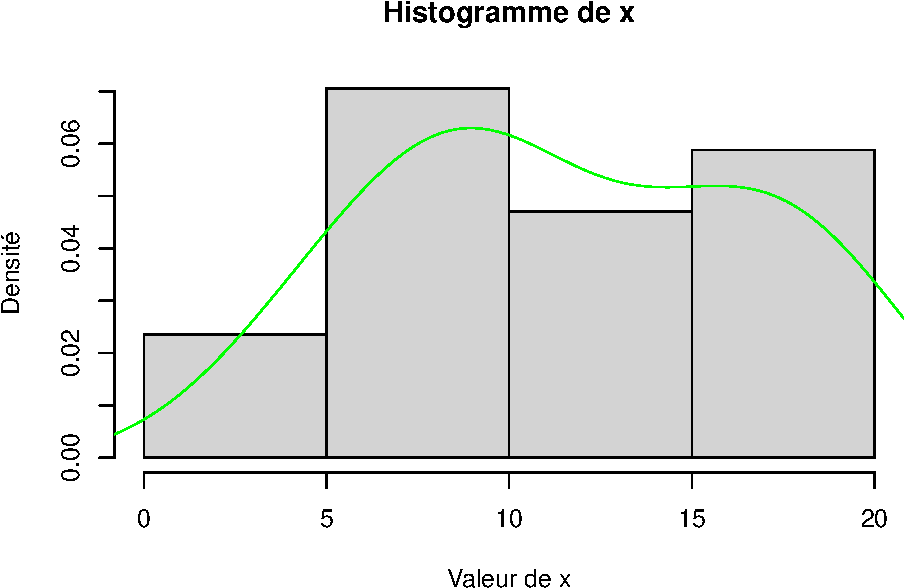
\includegraphics{_main_files/figure-latex/hist2-1.pdf}

On peut récupérer plus d'informations sur l'histogramme en affichant le résultat de la fonction \texttt{hist}.

\begin{Shaded}
\begin{Highlighting}[]
\CommentTok{\# Créer un vecteur de données}
\NormalTok{x }\OtherTok{\textless{}{-}} \FunctionTok{c}\NormalTok{(}\DecValTok{3}\NormalTok{, }\DecValTok{5}\NormalTok{, }\DecValTok{6}\NormalTok{, }\DecValTok{7}\NormalTok{, }\DecValTok{8}\NormalTok{, }\DecValTok{9}\NormalTok{, }\DecValTok{9}\NormalTok{, }\DecValTok{10}\NormalTok{, }\DecValTok{11}\NormalTok{, }\DecValTok{12}\NormalTok{, }\DecValTok{14}\NormalTok{, }\DecValTok{15}\NormalTok{, }\DecValTok{16}\NormalTok{, }\DecValTok{17}\NormalTok{, }\DecValTok{18}\NormalTok{, }\DecValTok{19}\NormalTok{, }\DecValTok{20}\NormalTok{)}

\CommentTok{\# Créer un histogramme avec 5 classes}
\NormalTok{hist }\OtherTok{\textless{}{-}} \FunctionTok{hist}\NormalTok{(x, }\AttributeTok{breaks =} \DecValTok{5}\NormalTok{, }\AttributeTok{freq=}\NormalTok{F, }\AttributeTok{main =} \StringTok{"Histogramme de x"}\NormalTok{, }\AttributeTok{ylab =} \StringTok{"Densité"}\NormalTok{, }\AttributeTok{xlab =} \StringTok{"Valeur de x"}\NormalTok{)}
\end{Highlighting}
\end{Shaded}

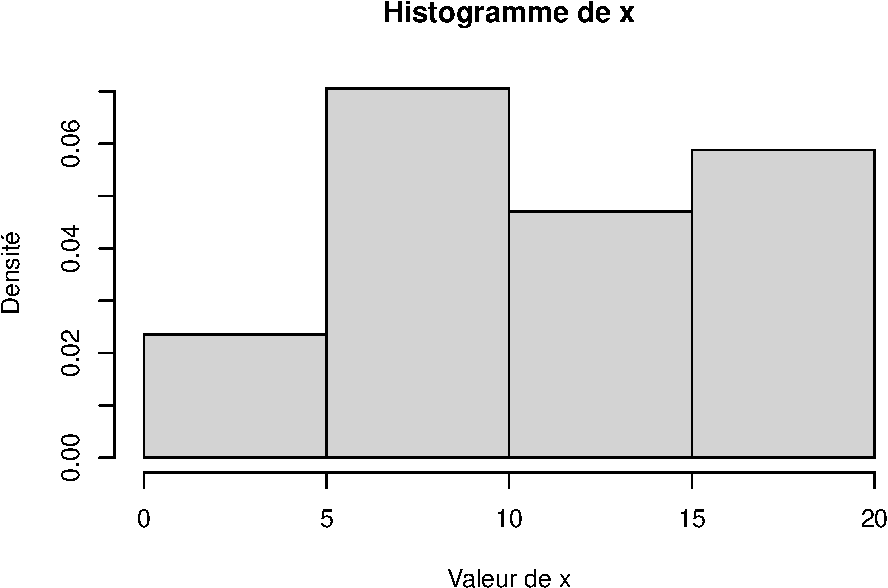
\includegraphics{_main_files/figure-latex/infos_hist2-1.pdf}

\begin{Shaded}
\begin{Highlighting}[]
\NormalTok{hist}
\end{Highlighting}
\end{Shaded}

\begin{verbatim}
## $breaks
## [1]  0  5 10 15 20
## 
## $counts
## [1] 2 6 4 5
## 
## $density
## [1] 0.02352941 0.07058824 0.04705882 0.05882353
## 
## $mids
## [1]  2.5  7.5 12.5 17.5
## 
## $xname
## [1] "x"
## 
## $equidist
## [1] TRUE
## 
## attr(,"class")
## [1] "histogram"
\end{verbatim}

Définition des valeurs sorties:

\begin{quote}
\$breaks: les bornes des intervalles\\
\$counts: le nombre de valeurs par intervalle\\
\$density: valeurs de la fonction de densité\\
\$mids: valeur centrale des intervalles\\
\$xname: nom de la variable x, tel qu'il est affiché sur le graphe\\
\$equidist: vrai si les intervalles sont équidistants
\end{quote}

\hypertarget{la-fonction-barplot}{%
\subsubsection{La fonction barplot()}\label{la-fonction-barplot}}

La fonction \texttt{barplot()} est utilisée pour créer un \textbf{graphique à barres}, également appelé un \textbf{diagramme à barres}. Le diagramme à barres est un graphique qui affiche des données catégorielles sous forme de barres rectangulaires, où la hauteur de chaque barre représente une \emph{mesure quantitative associée à cette catégorie}.

La fonction \texttt{barplot()} prend en entrée un vecteur ou une matrice de données, où chaque colonne représente une catégorie et chaque ligne représente une mesure quantitative pour cette catégorie. Les arguments optionnels peuvent être utilisés pour personnaliser le graphique, tels que les couleurs des barres, les étiquettes des axes, la légende, etc.

Voici un exemple d'utilisation de la fonction \texttt{barplot()} pour créer un graphique à barres à partir d'une matrice de données ``mat'':

\begin{Shaded}
\begin{Highlighting}[]
\CommentTok{\# Créer une matrice de données}
\NormalTok{mat }\OtherTok{\textless{}{-}} \FunctionTok{matrix}\NormalTok{(}\FunctionTok{c}\NormalTok{(}\DecValTok{2}\NormalTok{, }\DecValTok{3}\NormalTok{, }\DecValTok{5}\NormalTok{, }\DecValTok{4}\NormalTok{, }\DecValTok{6}\NormalTok{, }\DecValTok{8}\NormalTok{), }\AttributeTok{nrow =} \DecValTok{2}\NormalTok{, }\AttributeTok{byrow =} \ConstantTok{TRUE}\NormalTok{)}
\FunctionTok{rownames}\NormalTok{(mat) }\OtherTok{\textless{}{-}} \FunctionTok{c}\NormalTok{(}\StringTok{"Hommes"}\NormalTok{, }\StringTok{"Femmes"}\NormalTok{)}
\FunctionTok{colnames}\NormalTok{(mat) }\OtherTok{\textless{}{-}} \FunctionTok{c}\NormalTok{(}\StringTok{"Groupe A"}\NormalTok{, }\StringTok{"Groupe B"}\NormalTok{, }\StringTok{"Groupe C"}\NormalTok{)}

\CommentTok{\# Créer un graphique à barres}
\FunctionTok{barplot}\NormalTok{(mat, }\AttributeTok{main =} \StringTok{"Graphique à barres"}\NormalTok{, }\AttributeTok{xlab =} \StringTok{"Groupes"}\NormalTok{, }\AttributeTok{ylab =} \StringTok{"Mesures"}\NormalTok{, }
        \AttributeTok{col =} \FunctionTok{c}\NormalTok{(}\StringTok{"red"}\NormalTok{, }\StringTok{"blue"}\NormalTok{), }\AttributeTok{legend.text =} \FunctionTok{rownames}\NormalTok{(mat))}
\end{Highlighting}
\end{Shaded}

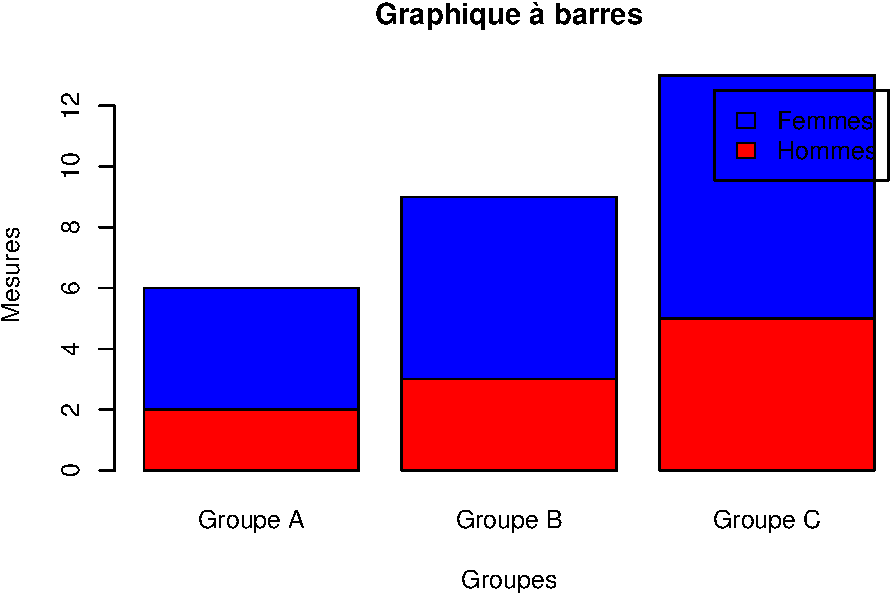
\includegraphics{_main_files/figure-latex/barplot-1.pdf}

Dans cet exemple, la fonction \texttt{barplot()} crée un graphique à barres à partir de la matrice de données \textbf{mat}. La fonction \texttt{rownames()} et \texttt{colnames()} sont utilisées pour nommer \emph{les lignes et les colonnes de la matrice}, qui seront utilisées comme \emph{étiquettes} d'axe dans le graphique. La fonction \texttt{barplot()} utilise les arguments optionnels pour personnaliser le graphique, tels que les couleurs des barres, les étiquettes des axes, la légende, etc.

\hypertarget{la-fonction-boxplot}{%
\subsubsection{La fonction boxplot()}\label{la-fonction-boxplot}}

La fonction \texttt{boxplot()} est utilisée pour créer un graphique en \textbf{boîte à moustache}. Le graphique affiche la \textbf{distribution d'un ensemble de données numériques à l'aide de cinq mesures statistiques : la médiane, les quartiles supérieurs et inférieurs, ainsi que les valeurs min et max}. Les ``moustaches'' représentent des \emph{intervalles de confiance} pour la distribution de données.

La fonction \texttt{boxplot()} prend en entrée un ou plusieurs vecteurs de données numériques, où chaque vecteur représente une variable à comparer. Les arguments optionnels peuvent être utilisés pour personnaliser le graphique, tels que les couleurs, les étiquettes des axes, la légende, etc.

Voici un exemple d'utilisation de la fonction \texttt{boxplot()} pour créer un boxplot à partir d'un vecteur de données ``x'':

\begin{Shaded}
\begin{Highlighting}[]
\CommentTok{\# Créer un vecteur de données}
\NormalTok{x }\OtherTok{\textless{}{-}} \FunctionTok{c}\NormalTok{(}\DecValTok{10}\NormalTok{, }\DecValTok{20}\NormalTok{, }\DecValTok{30}\NormalTok{, }\DecValTok{40}\NormalTok{, }\DecValTok{50}\NormalTok{, }\DecValTok{60}\NormalTok{, }\DecValTok{70}\NormalTok{, }\DecValTok{80}\NormalTok{, }\DecValTok{90}\NormalTok{, }\DecValTok{100}\NormalTok{)}

\CommentTok{\# Créer un graphique en boîte}
\FunctionTok{boxplot}\NormalTok{(x, }\AttributeTok{main =} \StringTok{"boîte à moustache"}\NormalTok{, }\AttributeTok{ylab =} \StringTok{"Valeurs"}\NormalTok{)}
\end{Highlighting}
\end{Shaded}

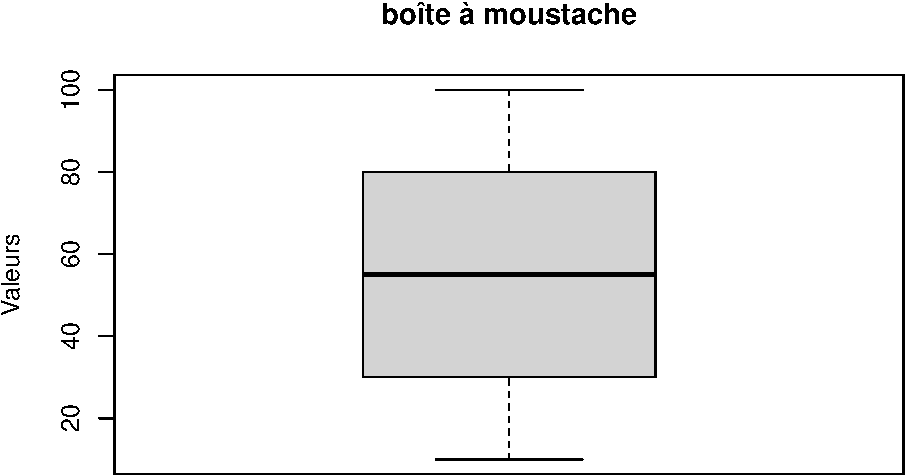
\includegraphics{_main_files/figure-latex/boxplot-1.pdf}

Dans cet exemple, la fonction \texttt{boxplot()} crée un graphique à partir du vecteur de données ``x''. La fonction utilise les arguments optionnels pour personnaliser le graphique, tels que le titre du graphique et l'étiquette de l'axe y. Les cinq mesures statistiques du vecteur de données sont représentées par la boîte et les moustaches. La boîte représente le quartile supérieur et le quartile inférieur, avec une ligne à l'intérieur représentant la médiane. Les moustaches représentent les valeurs minimum et maximum, avec des points éventuels représentant des valeurs aberrantes.

\hypertarget{les-fonctions-de-tracuxe9-de-courbes-de-niveau}{%
\subsubsection{Les fonctions de tracé de courbes de niveau}\label{les-fonctions-de-tracuxe9-de-courbes-de-niveau}}

Les fonctions de tracé de courbes de niveau permettent de \textbf{représenter des données en 3 dimensions sur un plan en deux dimensions}. Cela se fait en créant des courbes de niveau qui relient les points d'une surface ayant la même valeur.

Sous R, les fonctions de tracé de courbes de niveau les plus courantes sont \texttt{contour()} et \texttt{filled.contour()}.

La fonction \texttt{contour()} \textbf{trace des courbes de niveau} sur un graphique en deux dimensions. Elle prend en entrée une matrice de données ainsi que des arguments supplémentaires qui définissent le nombre et les niveaux de courbes de niveau à afficher.

La fonction \texttt{filled.contour()} \textbf{trace également des courbes de niveau, mais remplit les zones} entre les courbes de niveau avec des couleurs pour indiquer les variations de valeur de la surface. Cette fonction prend en entrée une matrice de données ainsi que des arguments supplémentaires qui définissent les niveaux et la palette de couleurs à utiliser pour remplir les zones entre les courbes de niveau.

Voici un exemple avec le jeu de données volcano qui contient des données topographiques sur le volcan Maunga Whau (New Zealand) selon une grille régulière de 10m x 10m.

\begin{Shaded}
\begin{Highlighting}[]
\FunctionTok{data}\NormalTok{(volcano)}
\CommentTok{\# Color palette}
\NormalTok{cols }\OtherTok{\textless{}{-}} \FunctionTok{hcl.colors}\NormalTok{(}\DecValTok{10}\NormalTok{, }\StringTok{"YlOrRd"}\NormalTok{)}
\FunctionTok{contour}\NormalTok{(volcano,}
        \AttributeTok{col =}\NormalTok{ cols)}
\end{Highlighting}
\end{Shaded}

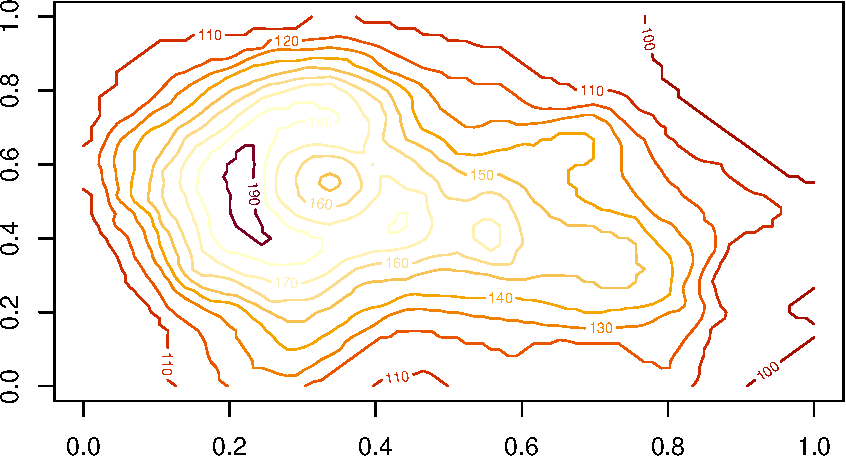
\includegraphics{_main_files/figure-latex/data_volcano-1.pdf}

\begin{Shaded}
\begin{Highlighting}[]
\FunctionTok{filled.contour}\NormalTok{(volcano,}
               \AttributeTok{nlevels =} \DecValTok{10}\NormalTok{)}
\end{Highlighting}
\end{Shaded}

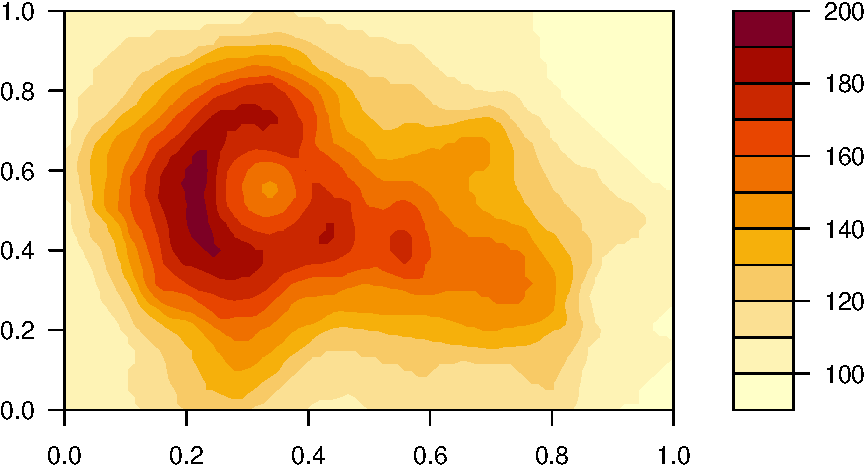
\includegraphics{_main_files/figure-latex/data_volcano-2.pdf}

\hypertarget{les-fonctions-de-cartographie}{%
\subsubsection{Les fonctions de cartographie}\label{les-fonctions-de-cartographie}}

Les fonctions cartographiques sous R permettent de créer et de manipuler des cartes géographiques. Voici quelques-unes des fonctions les plus couramment utilisées :

\begin{itemize}
\item
  \textbf{maps}: cette fonction permet de tracer des cartes géographiques en utilisant des données du package maps. Il est possible de personnaliser les couleurs, les frontières et les légendes de la carte.
\item
  \textbf{mapdata}: cette fonction permet de télécharger des données géographiques pour une région spécifique. Les données peuvent être utilisées pour tracer des cartes en utilisant la fonction maps.
\item
  \textbf{ggmap}: cette fonction permet de superposer des données sur des cartes géographiques provenant de Google Maps. Elle peut être utilisée pour créer des cartes interactives.
\item
  \textbf{ggplot2}: ce package offre de nombreuses fonctionnalités pour la création de cartes géographiques en utilisant la librairie ggplot2. Il permet de créer des cartes thématiques avec des couleurs et des symboles personnalisés.
\item
  \textbf{leaflet}: cette fonction permet de créer des cartes interactives à l'aide de la bibliothèque JavaScript Leaflet. Elle offre des options pour personnaliser les marqueurs, les popups et les couches de carte.
\item
  \textbf{raster}: cette fonction permet de manipuler des données raster telles que des images satellites et de créer des cartes à partir de ces données. Elle offre des fonctions pour la classification, la visualisation et la superposition de données raster.
\item
  \textbf{sp}: ce package offre des fonctionnalités pour la manipulation de données géographiques vectorielles. Il permet de créer des cartes thématiques et d'ajouter des données provenant de sources externes.
\end{itemize}

Ces fonctions cartographiques peuvent être combinées pour créer des cartes géographiques personnalisées et interactives en fonction des besoins de l'utilisateur.

\begin{Shaded}
\begin{Highlighting}[]
\FunctionTok{library}\NormalTok{(maps)}
\FunctionTok{library}\NormalTok{(mapdata)}
\FunctionTok{library}\NormalTok{(ggplot2)}

\CommentTok{\# Charger les données de population par ville}
\FunctionTok{data}\NormalTok{(}\StringTok{"world.cities"}\NormalTok{)}

\CommentTok{\# Extraire les villes françaises avec une population supérieure à 100 000}
\NormalTok{france.cities }\OtherTok{\textless{}{-}} \FunctionTok{subset}\NormalTok{(world.cities, country.etc }\SpecialCharTok{==} \StringTok{"France"} \SpecialCharTok{\&}\NormalTok{ pop }\SpecialCharTok{\textgreater{}} \DecValTok{100000}\NormalTok{)}

\CommentTok{\# Tracer la carte de la France}
\NormalTok{fr.map }\OtherTok{\textless{}{-}} \FunctionTok{map}\NormalTok{(}\AttributeTok{database =} \StringTok{"france"}\NormalTok{, }\AttributeTok{fill =} \ConstantTok{TRUE}\NormalTok{, }\AttributeTok{col =} \StringTok{"lightblue"}\NormalTok{, }\AttributeTok{bg =} \StringTok{"white"}\NormalTok{, }\AttributeTok{lty =} \DecValTok{0}\NormalTok{,}
    \AttributeTok{ylim =} \FunctionTok{c}\NormalTok{(}\DecValTok{40}\NormalTok{, }\DecValTok{54}\NormalTok{), }\AttributeTok{xlim =} \FunctionTok{c}\NormalTok{(}\SpecialCharTok{{-}}\DecValTok{5}\NormalTok{, }\DecValTok{10}\NormalTok{))}
\end{Highlighting}
\end{Shaded}

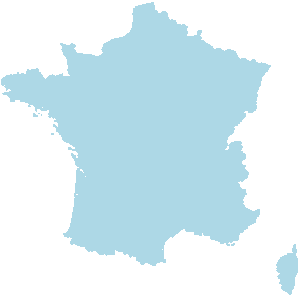
\includegraphics{_main_files/figure-latex/carto-1.pdf}

\begin{Shaded}
\begin{Highlighting}[]
\CommentTok{\# Créer un graphique ggplot avec la carte de la France}
\CommentTok{\# Ajouter des cercles proportionnels pour chaque ville en fonction de leur population}
\FunctionTok{ggplot}\NormalTok{() }\SpecialCharTok{+}
  \FunctionTok{geom\_polygon}\NormalTok{(}\AttributeTok{data =}\NormalTok{ fr.map, }\FunctionTok{aes}\NormalTok{(}\AttributeTok{x =}\NormalTok{ long, }\AttributeTok{y =}\NormalTok{ lat, }\AttributeTok{group =}\NormalTok{ group), }
               \AttributeTok{fill =} \StringTok{"lightblue"}\NormalTok{, }\AttributeTok{color =} \StringTok{"black"}\NormalTok{) }\SpecialCharTok{+}
  \FunctionTok{geom\_point}\NormalTok{(}\AttributeTok{data =}\NormalTok{ france.cities, }\FunctionTok{aes}\NormalTok{(}\AttributeTok{x =}\NormalTok{ long, }\AttributeTok{y =}\NormalTok{ lat, }\AttributeTok{size =}\NormalTok{ pop), }
             \AttributeTok{color =} \StringTok{"red"}\NormalTok{, }\AttributeTok{alpha =} \FloatTok{0.8}\NormalTok{) }\SpecialCharTok{+}
  \FunctionTok{labs}\NormalTok{(}\AttributeTok{size =} \StringTok{"Taille de la population"}\NormalTok{)}\SpecialCharTok{+}
  \FunctionTok{coord\_fixed}\NormalTok{(}\AttributeTok{xlim =} \FunctionTok{c}\NormalTok{(}\SpecialCharTok{{-}}\DecValTok{5}\NormalTok{, }\DecValTok{10}\NormalTok{), }\AttributeTok{ylim =} \FunctionTok{c}\NormalTok{(}\DecValTok{40}\NormalTok{, }\DecValTok{54}\NormalTok{)) }\SpecialCharTok{+}
  \FunctionTok{scale\_size\_continuous}\NormalTok{(}\AttributeTok{range =} \FunctionTok{c}\NormalTok{(}\DecValTok{1}\NormalTok{, }\DecValTok{10}\NormalTok{)) }
\end{Highlighting}
\end{Shaded}

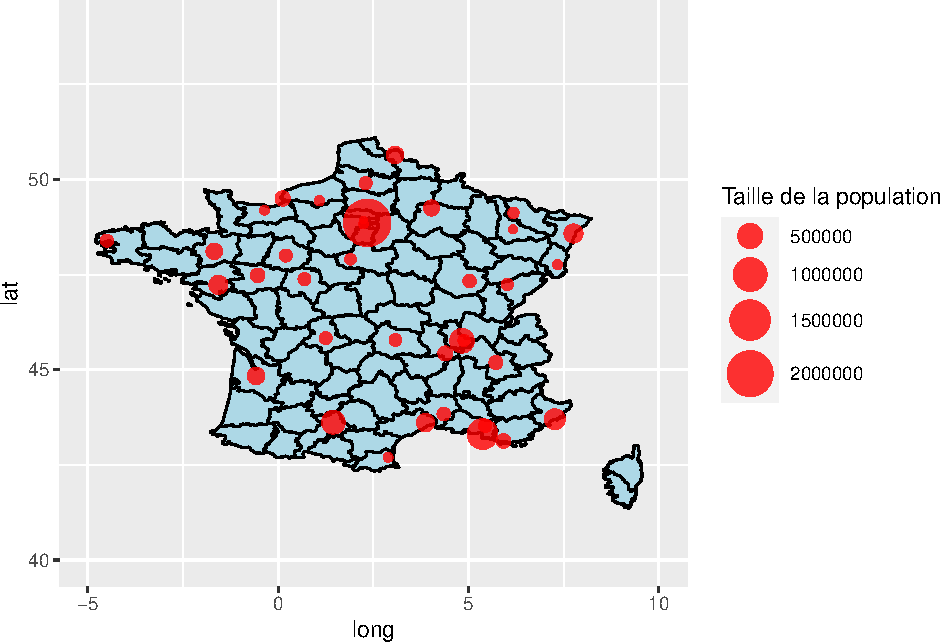
\includegraphics{_main_files/figure-latex/carto-2.pdf}

\textbf{Exercice 4:}

\begin{enumerate}
\def\labelenumi{\arabic{enumi}.}
\item
  Créez un graphique en nuage de points pour représenter la relation entre le poids et la consommation de carburant de différentes voitures en utilisant le jeu de données mtcars.
\item
  Créez un graphique en barres empilées pour représenter la répartition des espèces de fleurs dans le jeu de données iris.
\item
  Créez un graphique en boîtes pour comparer les espérances de vie dans différents pays dans le jeu de données gapminder.
\item
  Créez un graphique en secteurs pour représenter la répartition des habitants par continent dans le jeu de données gapminder.
\end{enumerate}

\hypertarget{references}{%
\section{References}\label{references}}

  \bibliography{book.bib,packages.bib}

\end{document}
